\chapter{Implementation}

%The implementation should look at any issues you encountered as you tried to implement your design. During the work, you might have found that elements of your design were unnecessary or overly complex, perhaps third party libraries were available that simplified some of the functions that you intended to implement. If things were easier in some areas, then how did you adapt your project to take account of your findings?

%It is more likely that things were more complex than you first thought. In particular, were there any problems or difficulties that you found during implementation that you had to address? Did such problems simply delay you or were they more significant? Your implementation might well be described in the same chapter as Problems (see below).

\section{Prototype}
Building a prototype will quickly highlight the main flaws in the initial design.  This is not the same as the intended final version and in this case is not even the same materials as I have chosen.  It does however confirm the basic design but is made from much cheaper sourced components.  I already had an Arduino Uno (the basic prototyping model) from my interest in the technology before I attended university, so this was an easy component to acquire quickly and is perfect for a prototype.  I had no chassis built or any materials to make one so I found a cheap and easy to assemble one online at a hobbyist electronics retailer.  This kit also included some very small DC motors with gearboxes and wheels, very convenient little package.  The Arduino along with the chassis kit and a small infrared sensors, a 9 volt battery and some jumper wires and a prototype was put together in a short period of time.
\begin{figure}[H]
\centering
        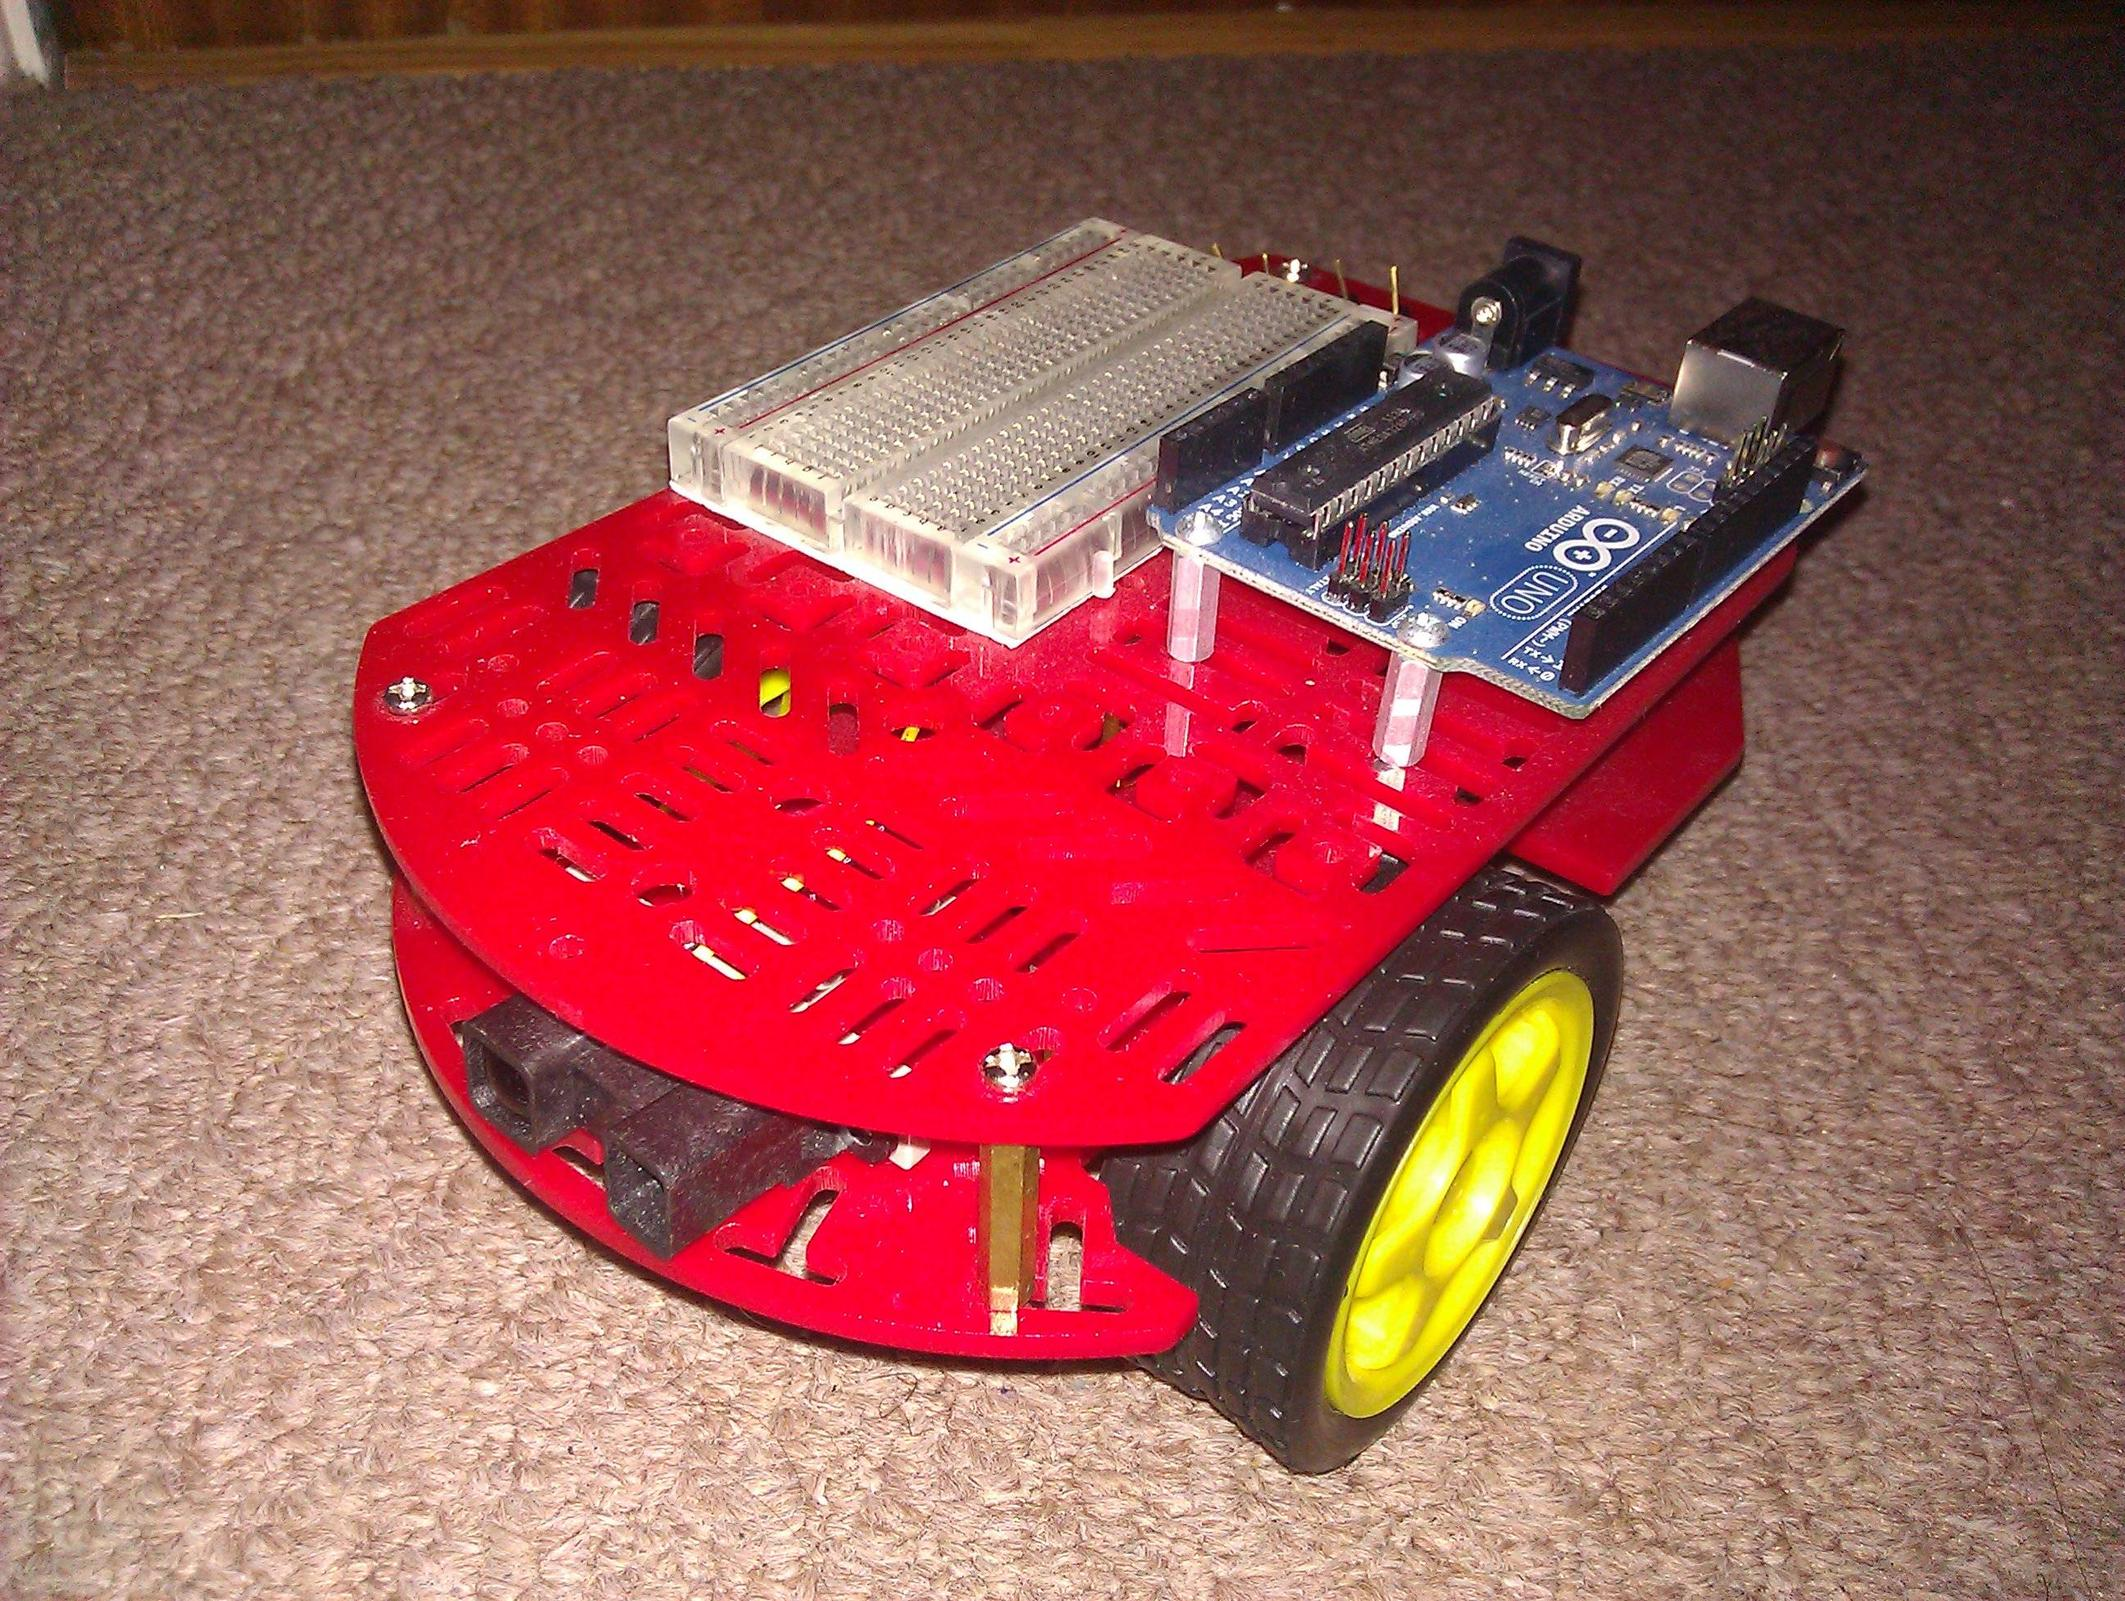
\includegraphics[width=3.0in] {Images/tria-mkI.jpg}
        \caption{Prototype mkI}
        \label{Prototype mkI}
\end{figure}

Wiring up the components was fairly easy due to there only being two motors and a single infrared sensor.  The sensor just has 3 pins, ground and positive power pins as well as a signal pin.  This is basically set up like a resistor, you supply power to the positive pin, attach the ground to the ground power rail of the system and just read the value being transmitted back on the signal pin.  The difference between zero up to the amount of power being given to the sensor, in this case the data sheet specified 5 volts as the upper edge and that is what I supplied the sensor with, gives an indication of how far it is from an object.  With this sensor the higher value returned is actually how close the object is and the lower number indicates it is further away.  This is due to the fact that the reading received is indicating how intense the amount of infrared getting back to the sensor is.
\\The harder part of this was getting the motors to run safely, this issue was discovered when putting together this prototype and testing each part as it was implemented.  The Arduino I use for prototyping can only output a regulated voltage of 3.3 or 5 volts.  The motors supplied with the chassis kit do not run very well at this voltage and struggle to move on thick carpet.  As the supply I am using to power the Arduino is a 9 volt battery this was sufficient to run the motors at an acceptable level, the only problem is supplying this to both the Arduino and the motors.  As the microcontroller is needed to control when and how fast the motors are to turn, simply wiring the power supply directly to the motors is a bad idea as they will just spin constantly due to always having power.
\begin{figure}[H]
\centering
        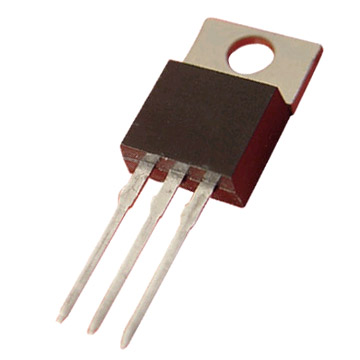
\includegraphics[width=2.0in] {Images/transistor.jpg}
        \caption{Transistor - zmescience.com}
        \label{Transistor}
\end{figure}

This could be solved using a transistor (a semiconductor device used to switch electrical signals) by supplying it with the higher voltage, connecting it to the motor and when a signal voltage from the Arduino is received it switches to the higher voltage allowing the motor to turn.  This is a very handy little component which is at the core of modern day electronics, but to use it in this fashion would need a lot more complicated circuitry as to ensure that this higher voltage does not damage other components in the circuit.  Another solution would be to use a chip known as a h-bridge.
\\This chip also acts like a switch but with the addition that it can change the currents direction meaning that you can not only control when the motor is on or off but also the direction it turns without additional complex circuitry.
\begin{figure}[H]
\centering
	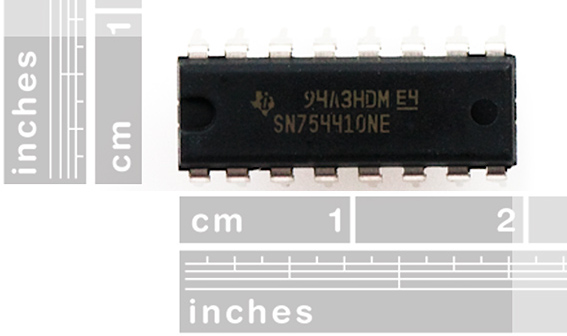
\includegraphics[width=2.0in]  {Images/h-bridge.jpg}
	\caption{H-Bridge - sparkfun.com}
	\label{H-Bridge}
\end{figure}
I discovered that the h-bridge chip also has its issues, as it generates heat when high currents are passed through it so if the motors are working hard more current will be drawn and the more heat the chip will generate and possibly burn out.  There is again the issue of having no protection for the rest of the circuit.  An option that would solve this issue is a full motor driver board but the cost if these is many times the cost of the components to make the circuits myself.  For example a h-bridge chip an assortment of diodes, capacitors, resistors and transistors costs around \pounds5 while a fully built board costs around \pounds20-30.
\begin{figure}[H]
\centering
        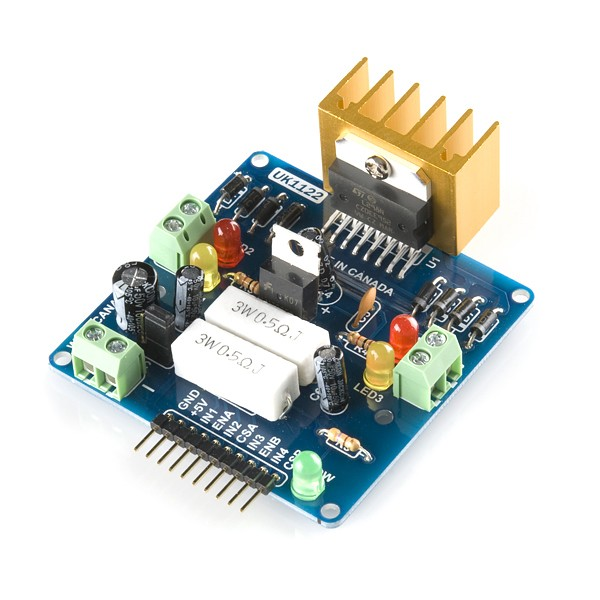
\includegraphics[width=2.0in]  {Images/motor-driver.jpg}
        \caption{Motor Driver - sparkfun.com}
        \label{Motor Driver}
\end{figure}
I decided to build a simple motor driver using the h-bridge chips, effective for a simple prototype.
\\With only a single infrared sensor the only logical place to mount it would be to have it facing directly forwards.  After writing the code to control the motors and process readings taken from the front mounted sensor the logic to test the concept is very simple.  Just check if there is something close in front and if there is just turn and check again, if there is not just keep moving forwards.
The logic looks like this:
\begin{figure}[H]
\begin{lstlisting}[basicstyle=\ttfamily]
if(sensor_range < value)
{
	motors.turn.right(45);
}else
{
	motors.move.forward(1);
}
\end{lstlisting}
\caption{Prototype Code Exert}
\label{Prototype Code Exert}
\end{figure}
This seems to work quite well, it does drive forwards and it does turn when an object comes in range of the infrared sensor.  This is the desired behaviour but there is a problem.  If the robot turns away from one object and into another, if that second object is too close by the time it comes in front of the sensor then it can not be seen by the sensor.  The sensor that I have fitted to the prototype has a maximum range of 150cm, but it also has a minimum range of 20cm meaning that is blind to any object closer than this minimum range.
\\In the figure the red signifies the blind area of the sensor and the green is the visible area.  If the robot were to turn right to avoid the wall in front of it then it would collide with the other wall and not be able to detect it.
\begin{figure}[H]
\centering
        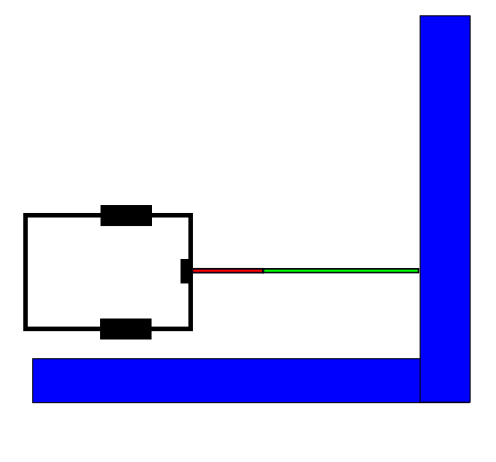
\includegraphics[width=3.0in]  {Images/ir-demo.png}
        \caption{Collision Illustration}
        \label{Collision Illustration}
\end{figure}
Another issue with the prototype robot is with the motors.  Even though I am supplying each motor with the same voltage they do not turn at the same speed, this is due to the lack of feedback with controlling them.  Also the fact that it is built from a very cheap kit is a probable reason for how uneven the speed of the motors is.  This all leads to the robot driving in a curve as opposed to the intended straight line, also contributing to the sensor problem of turning into an object putting it within the sensor blind spot.
\subsection{Prototype Evaluation}
The main issues with the prototype are the motors and the lack of more than a single sensor.
\\The motors did not run at exactly the same speed causing the robot to turn constantly as well as having no feedback system connected to the motors or the wheels and as such the robot nor the user know what position the drive system is in or how far the robot has moved.
\\Having just a single sensor facing directly forwards highlighted the need for more sensors covering a wider area in front of the robot due to when turning objects may be moved into the blind spot of the sensor and not be seen causing a collision.
\\These issues were taken into consideration when designing the second iteration of the robot.

\section{MK-I}
The next step was to build a version based on the design and using the things that were learnt from the prototype to improve it.
\\First thing to do was to build a sturdy chassis for all the systems to be mounted onto.  I bought several sheets of aluminium to but cut into a similar shape as the small red plastic prototype.
\begin{figure}[H]
\centering
        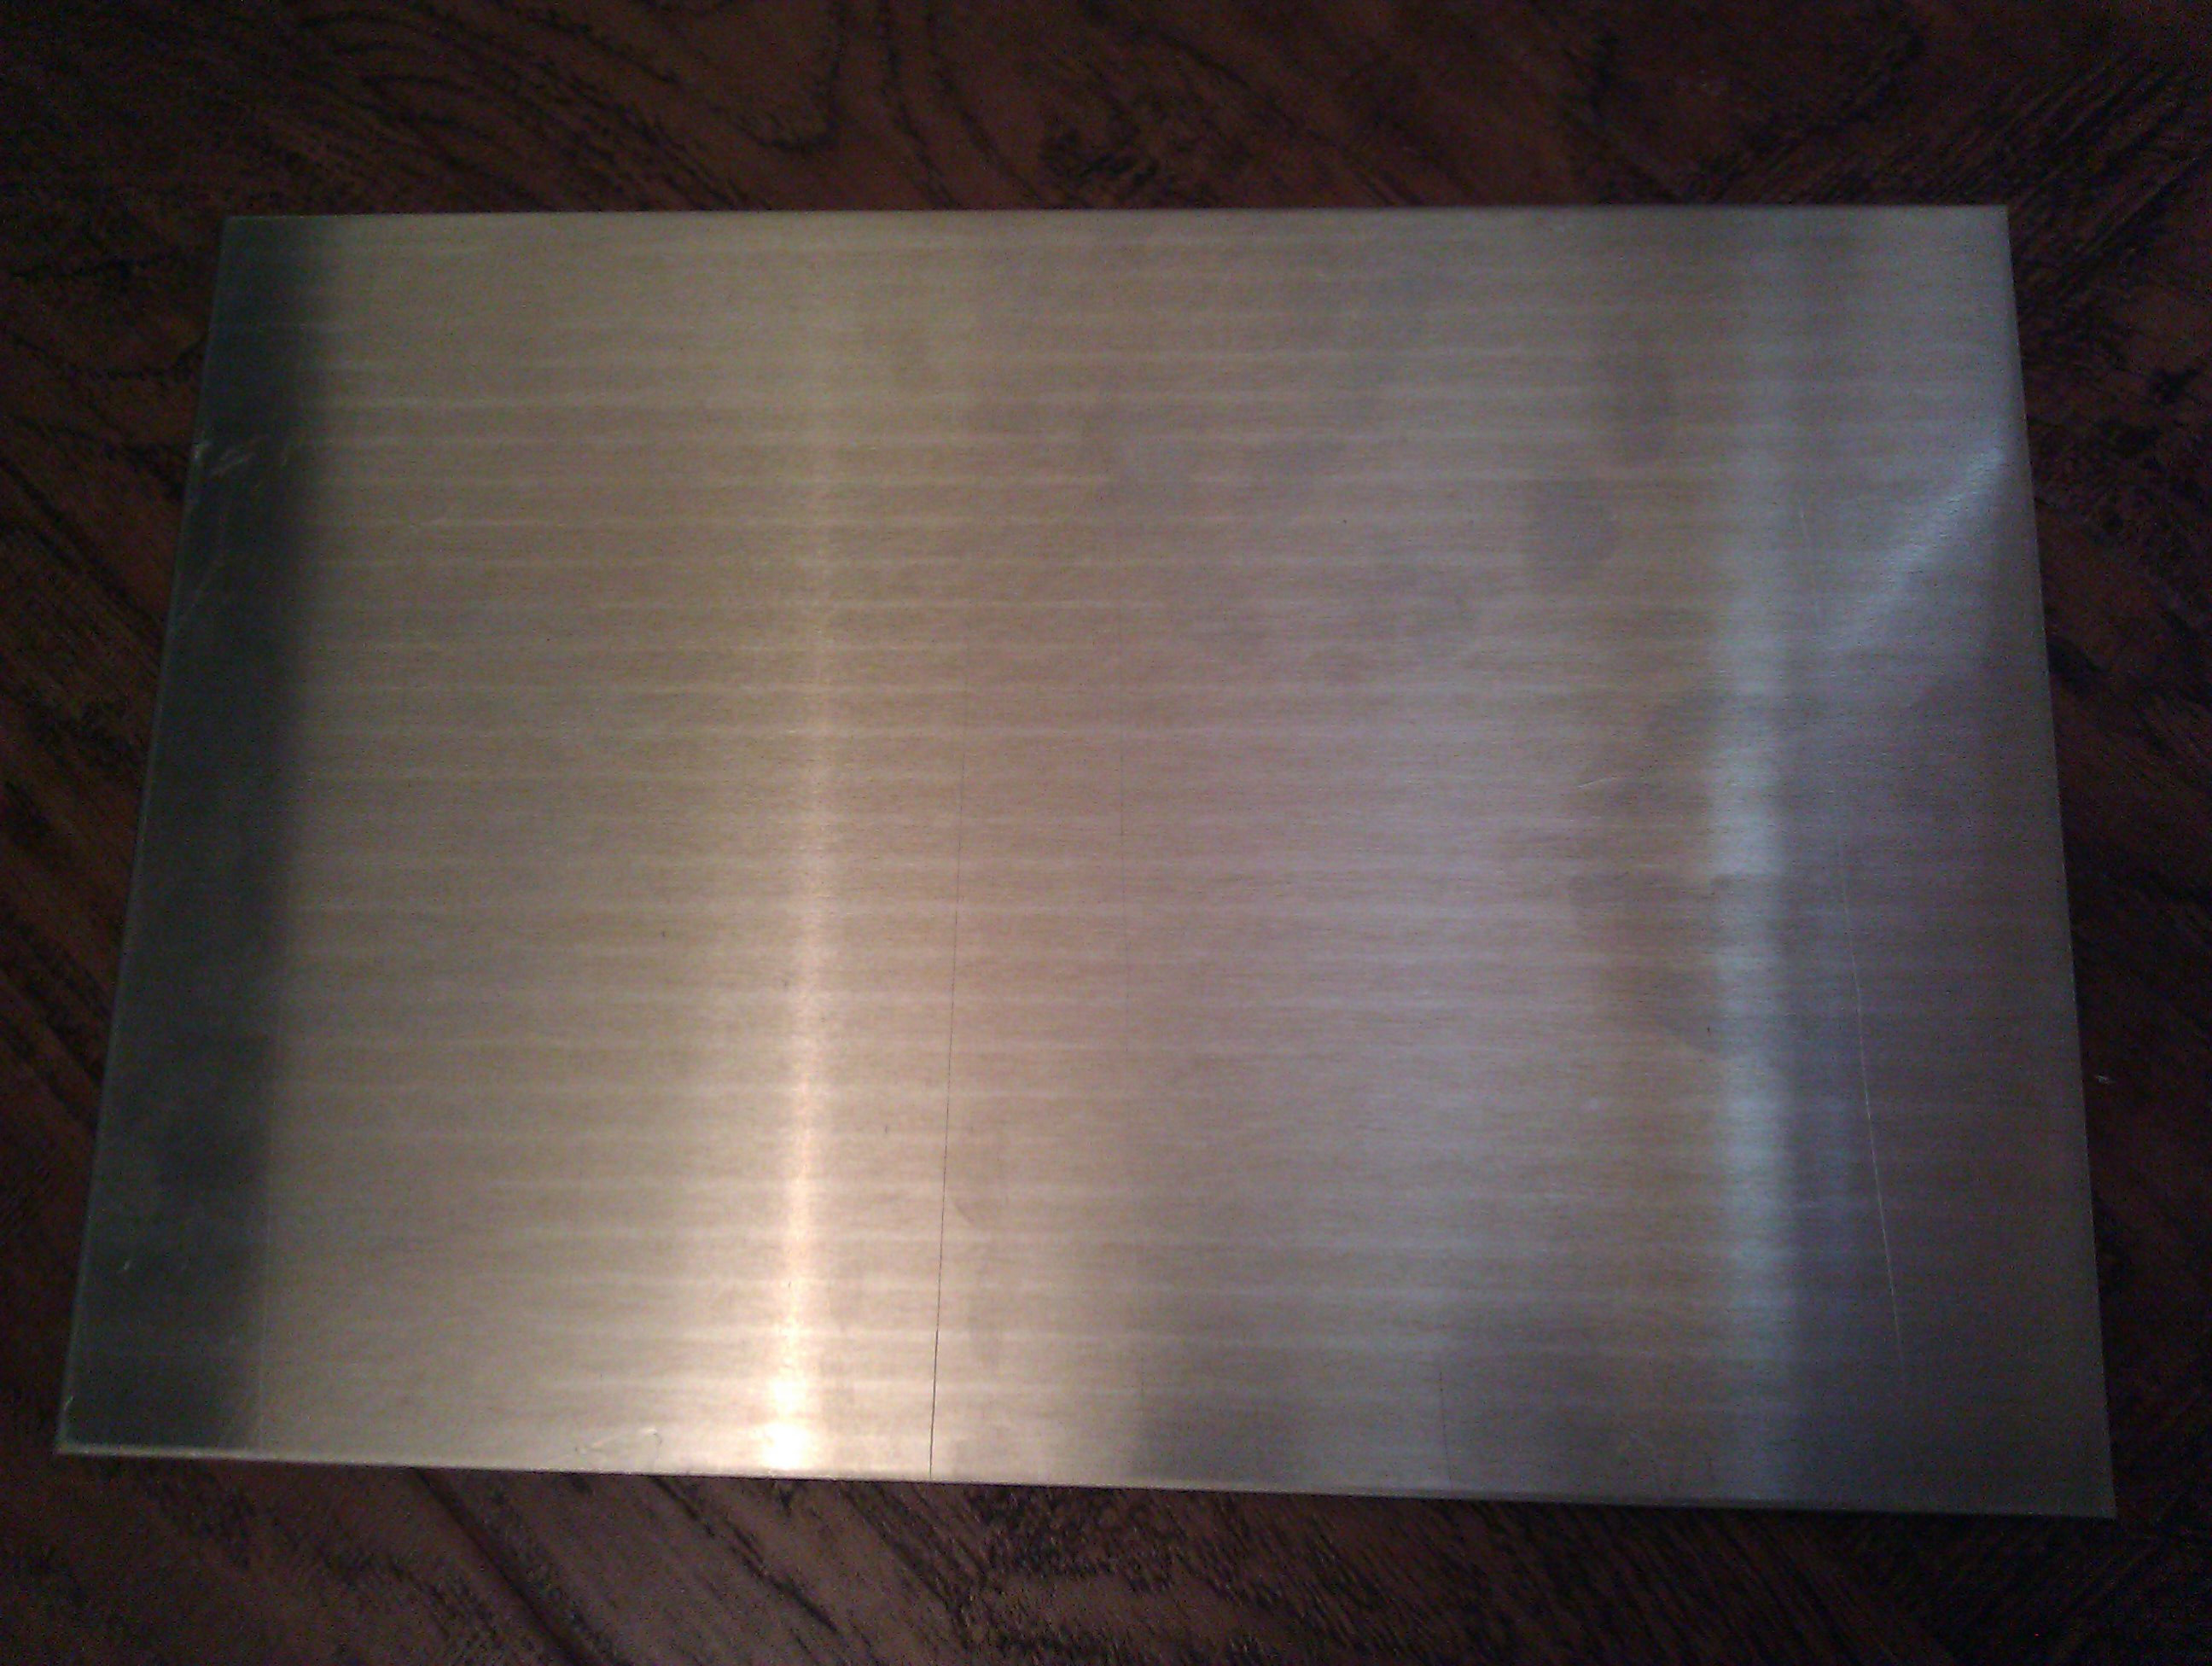
\includegraphics[width=3.0in]  {Images/alu-sheet-2.jpg}
        \caption{Aluminium Sheet}
        \label{Aluminium Sheet}
\end{figure}
I chose this shape mainly because of how much I liked working with the kit used in making the prototype.  Even though the first version was not perfect, the sensor was successful to a certain degree, it just needed more of them to cover the blind spots.  The curved shape of the front where the sensors mounted makes sense because then each sensor reading will provide the same relative distance from the robot unlike if it was square than the edge would be closer to the object in the environment than the robot thinks.
\begin{figure}[H]
\centering
        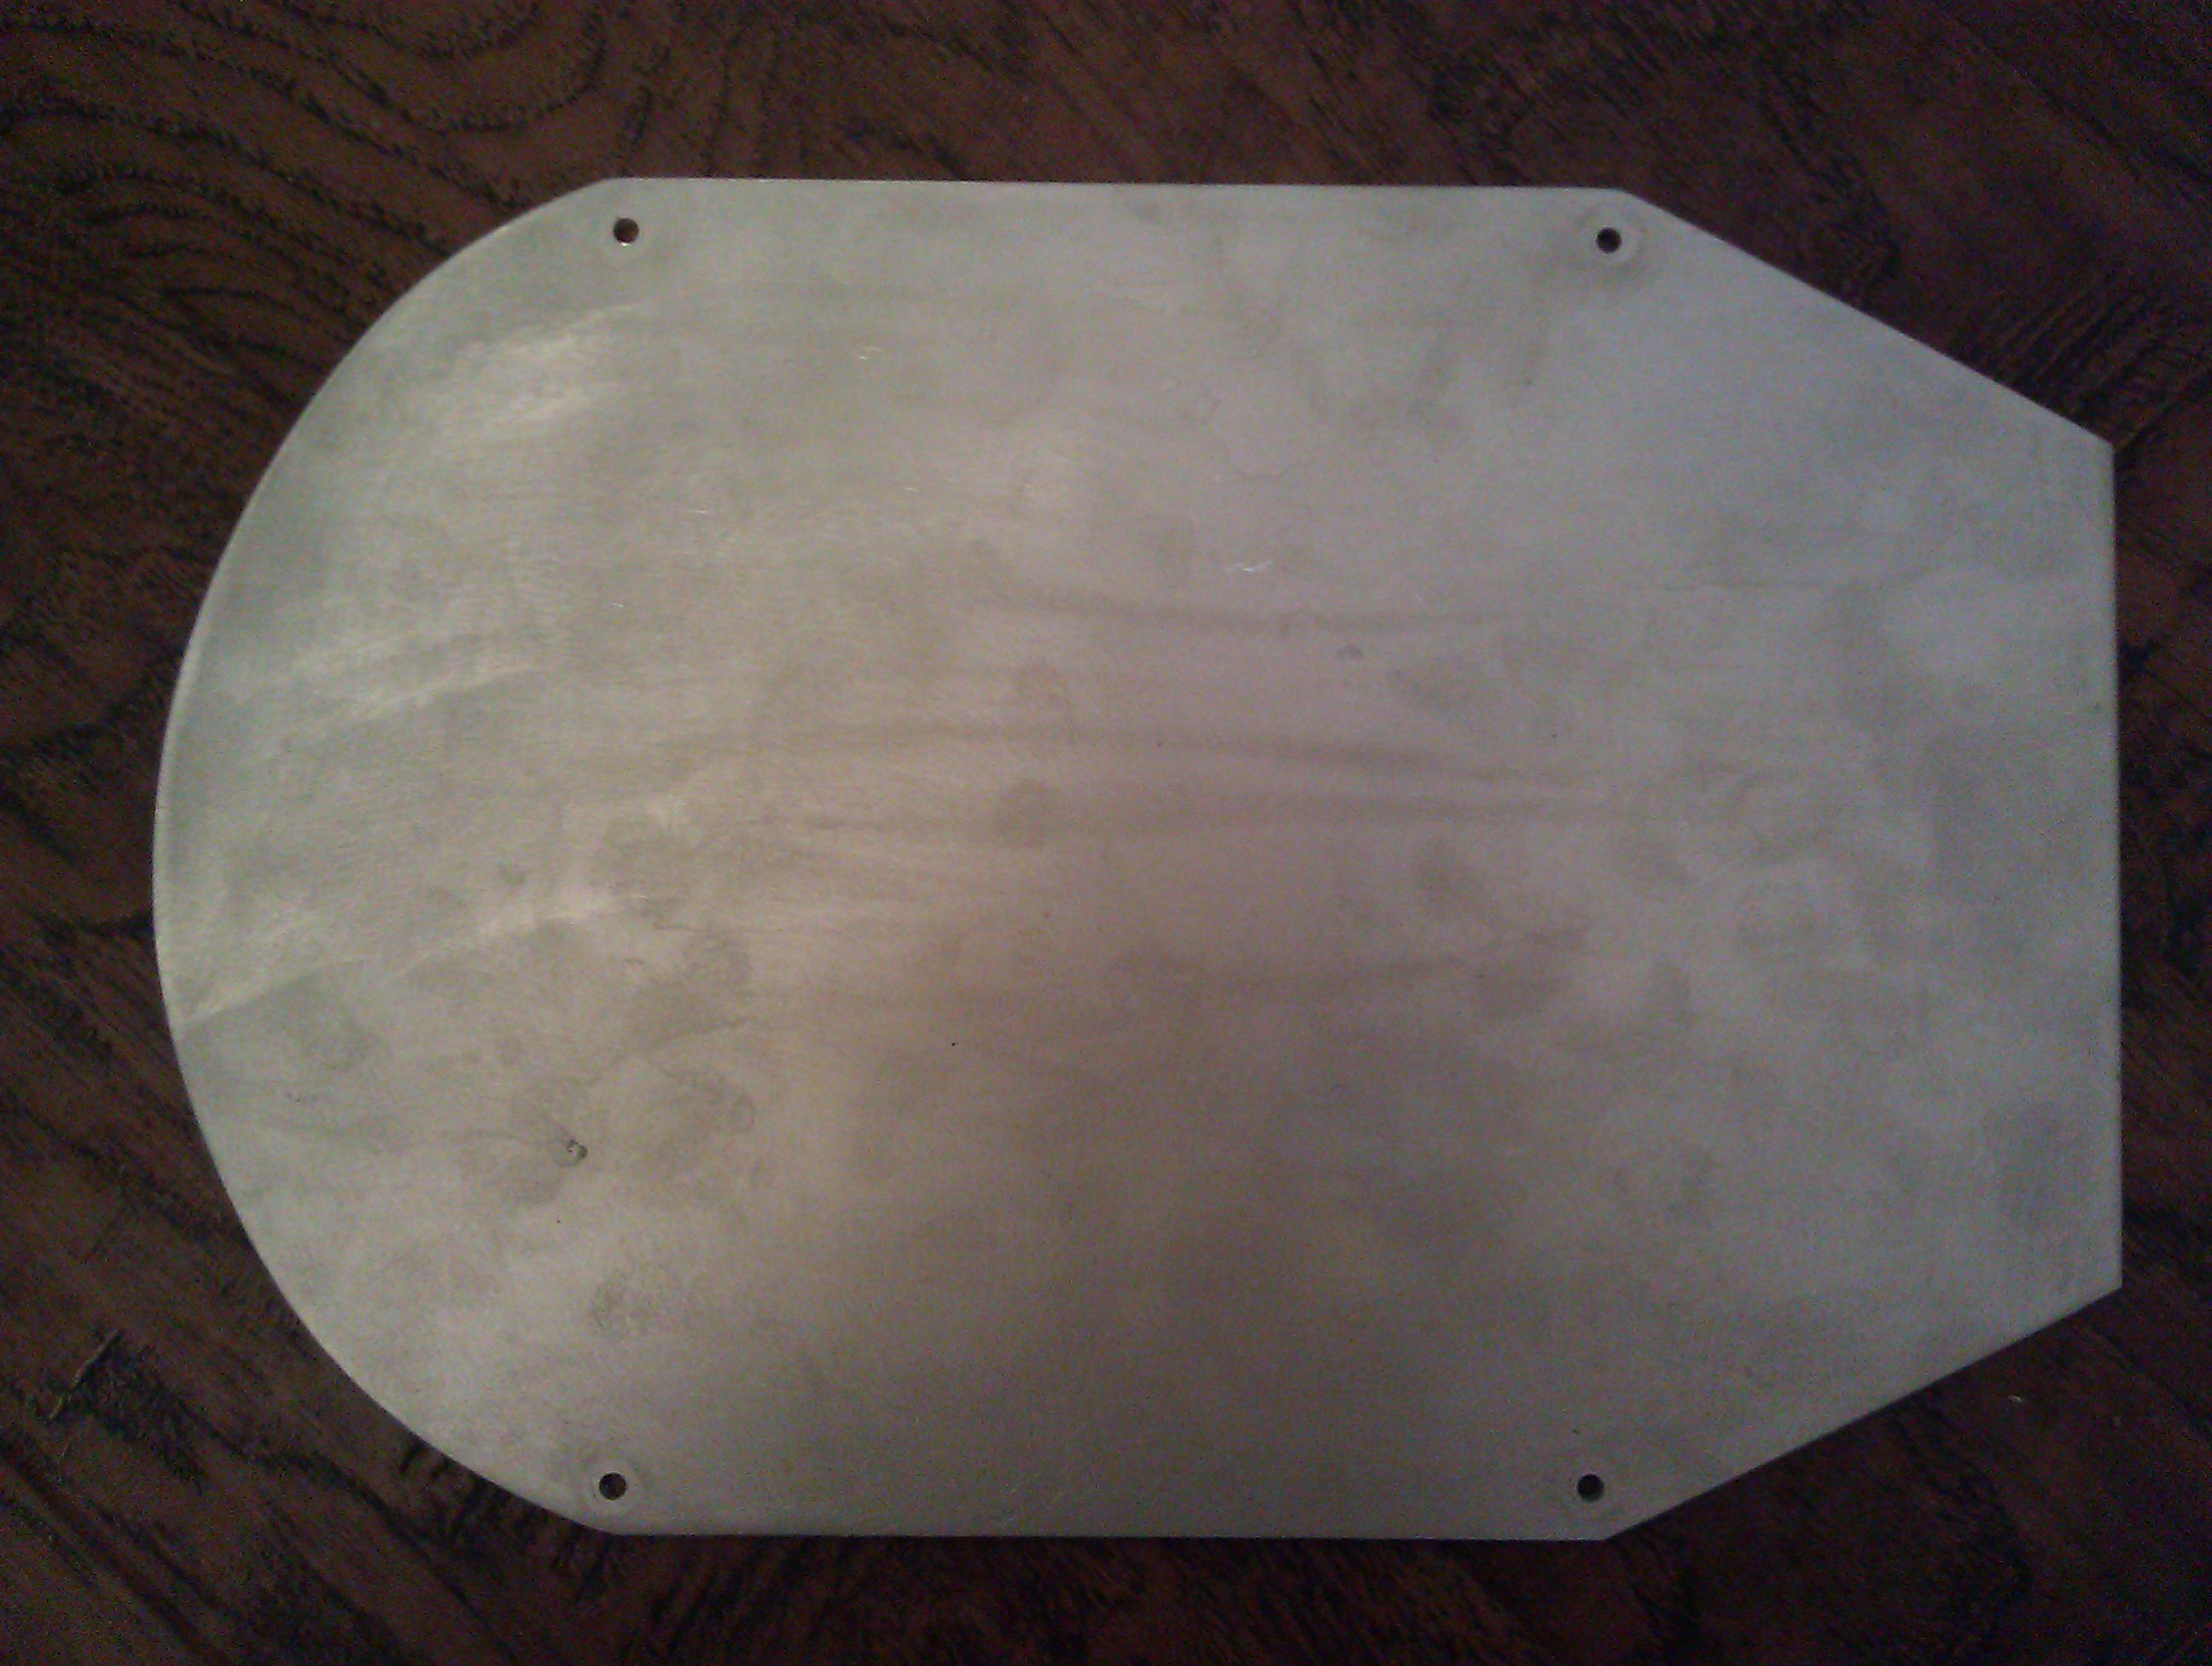
\includegraphics[width=3.0in]  {Images/alu-cut-2.jpg}
        \caption{Aluminium Sheet Cut}
        \label{Aluminium Sheet Cut}
\end{figure}
Next was to think about how to mount the motors to this aluminium base plate. After measuring the size of the stepper motors I bought to use as part of the robots drive system I also purchased a strip of aluminium to be cut and shaped into a motor mount to be attached on the underside of the baseplate.
\begin{figure}[H]
\centering
        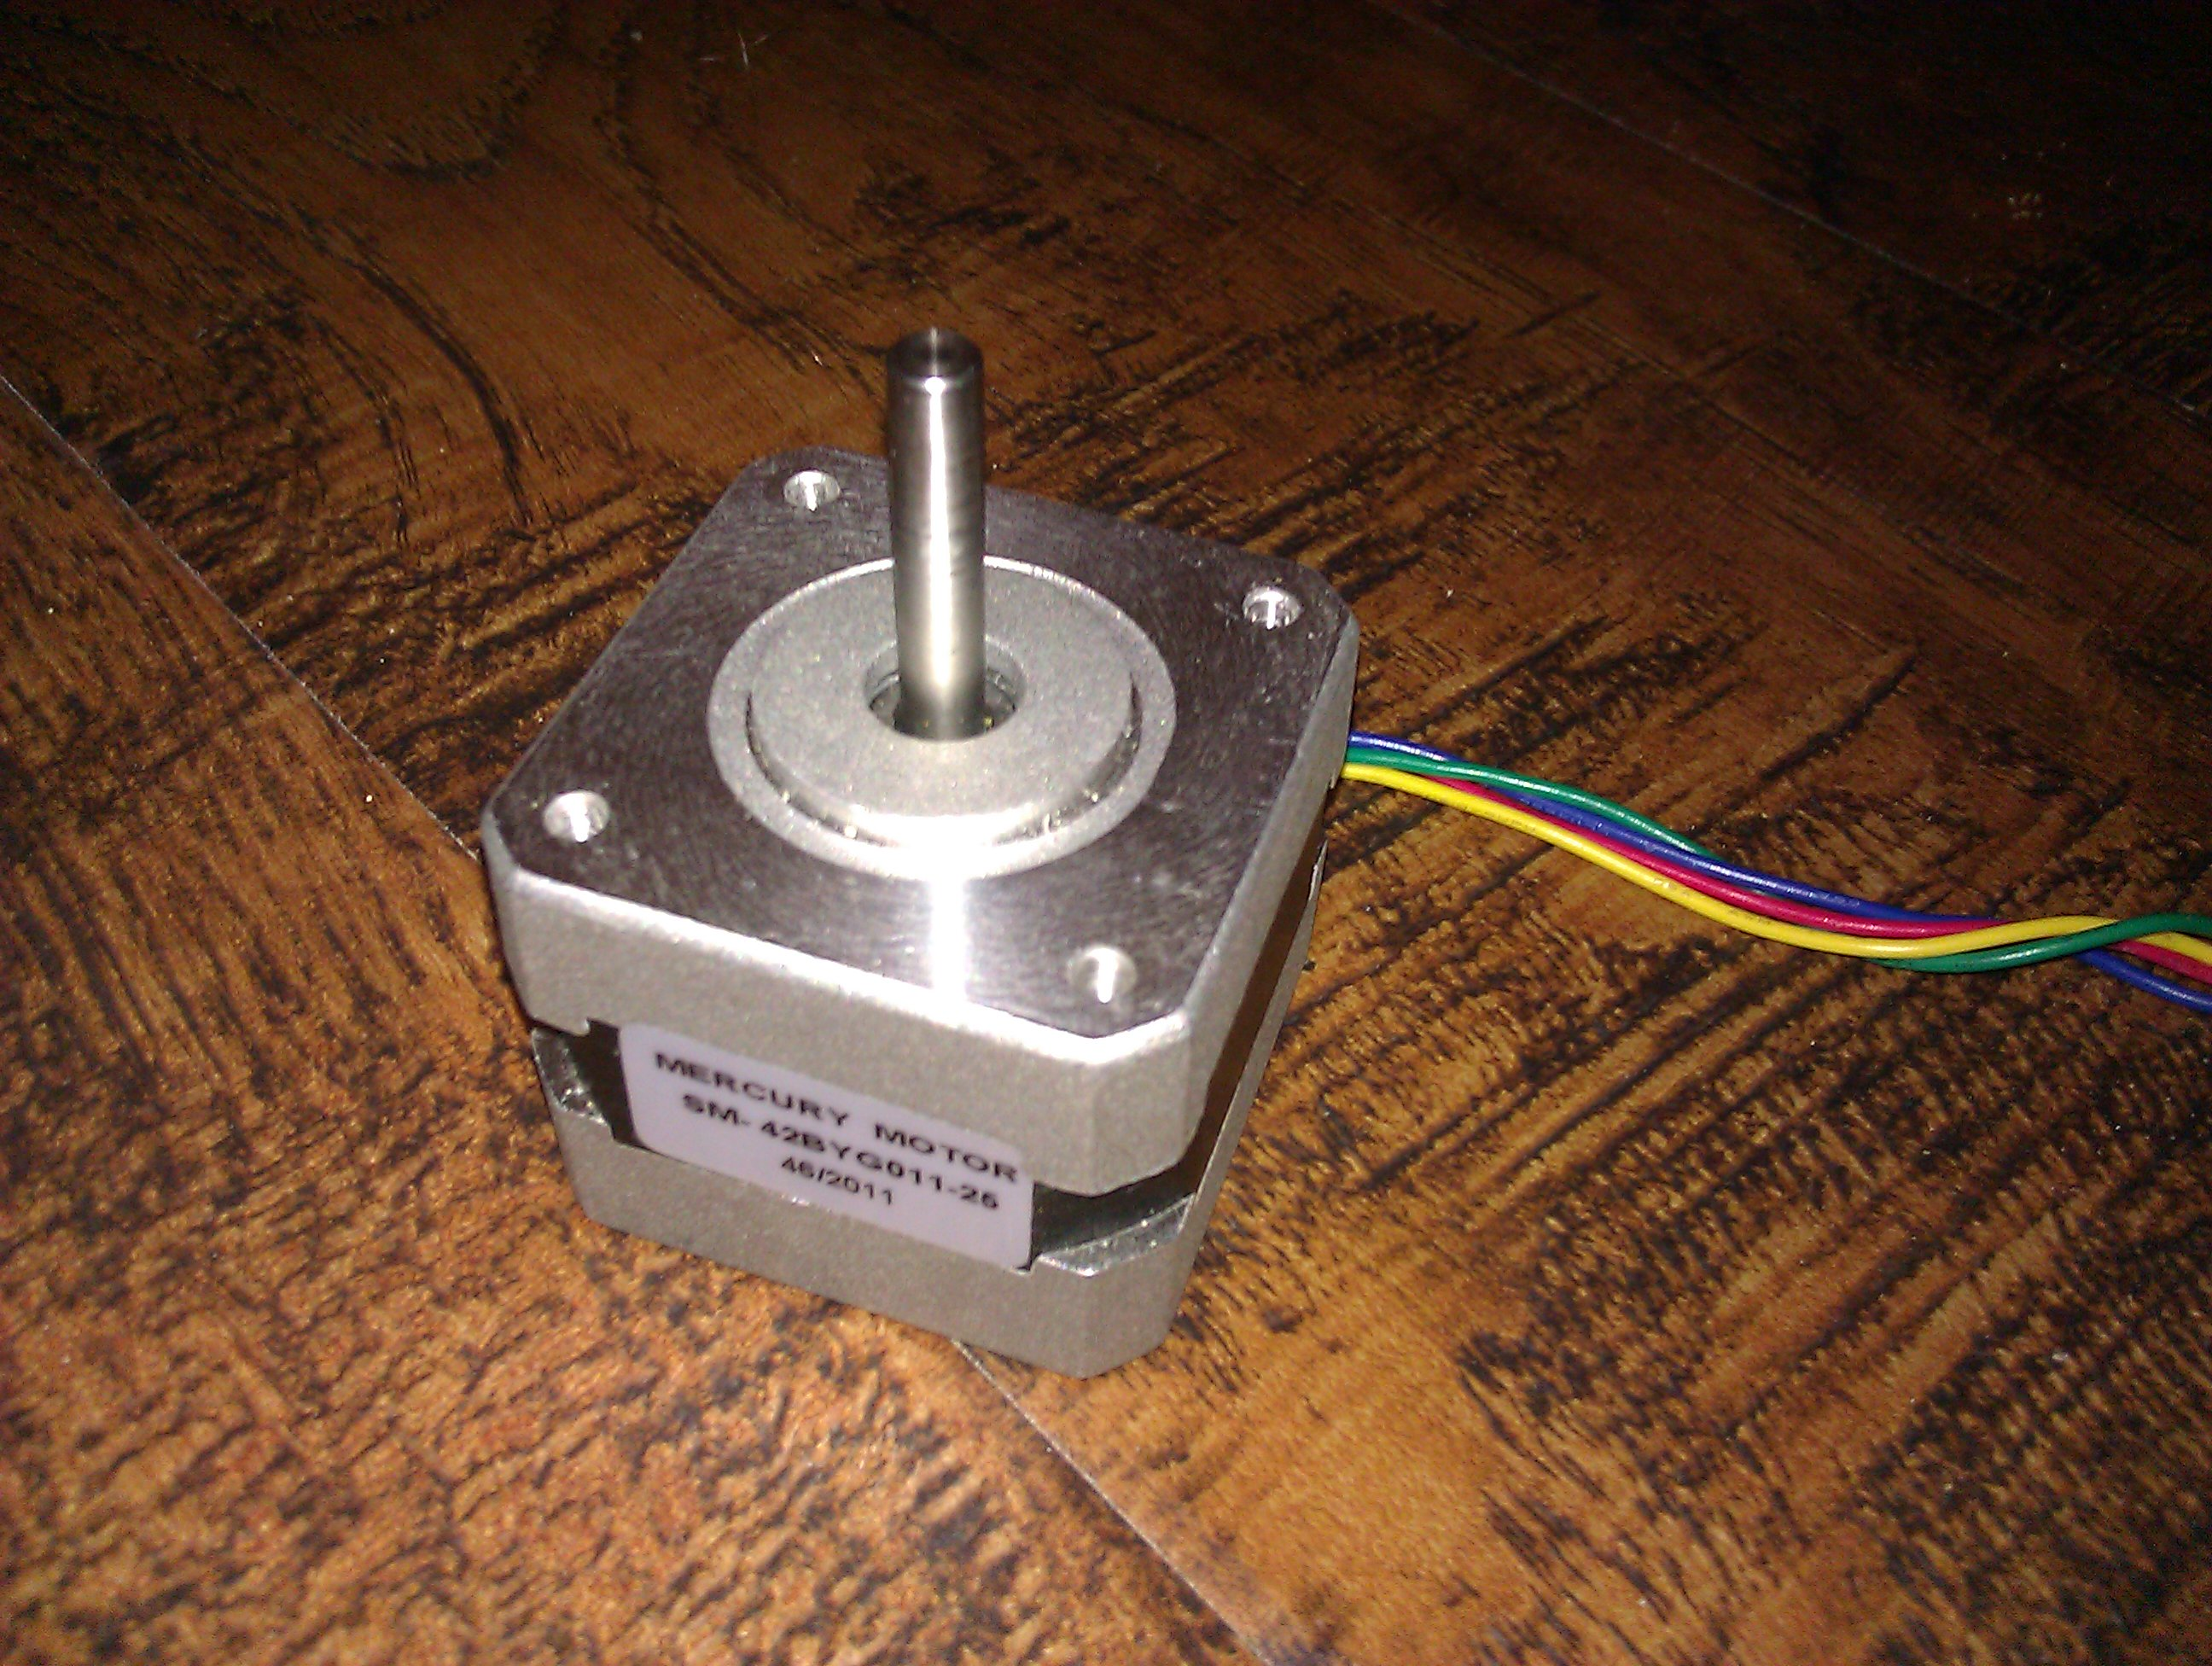
\includegraphics[width=3.0in]  {Images/small-stepper.jpg}
        \caption{Chosen Stepper Motor}
        \label{Chosen Stepper Motor}
\end{figure}
\begin{figure}[H]
\centering
        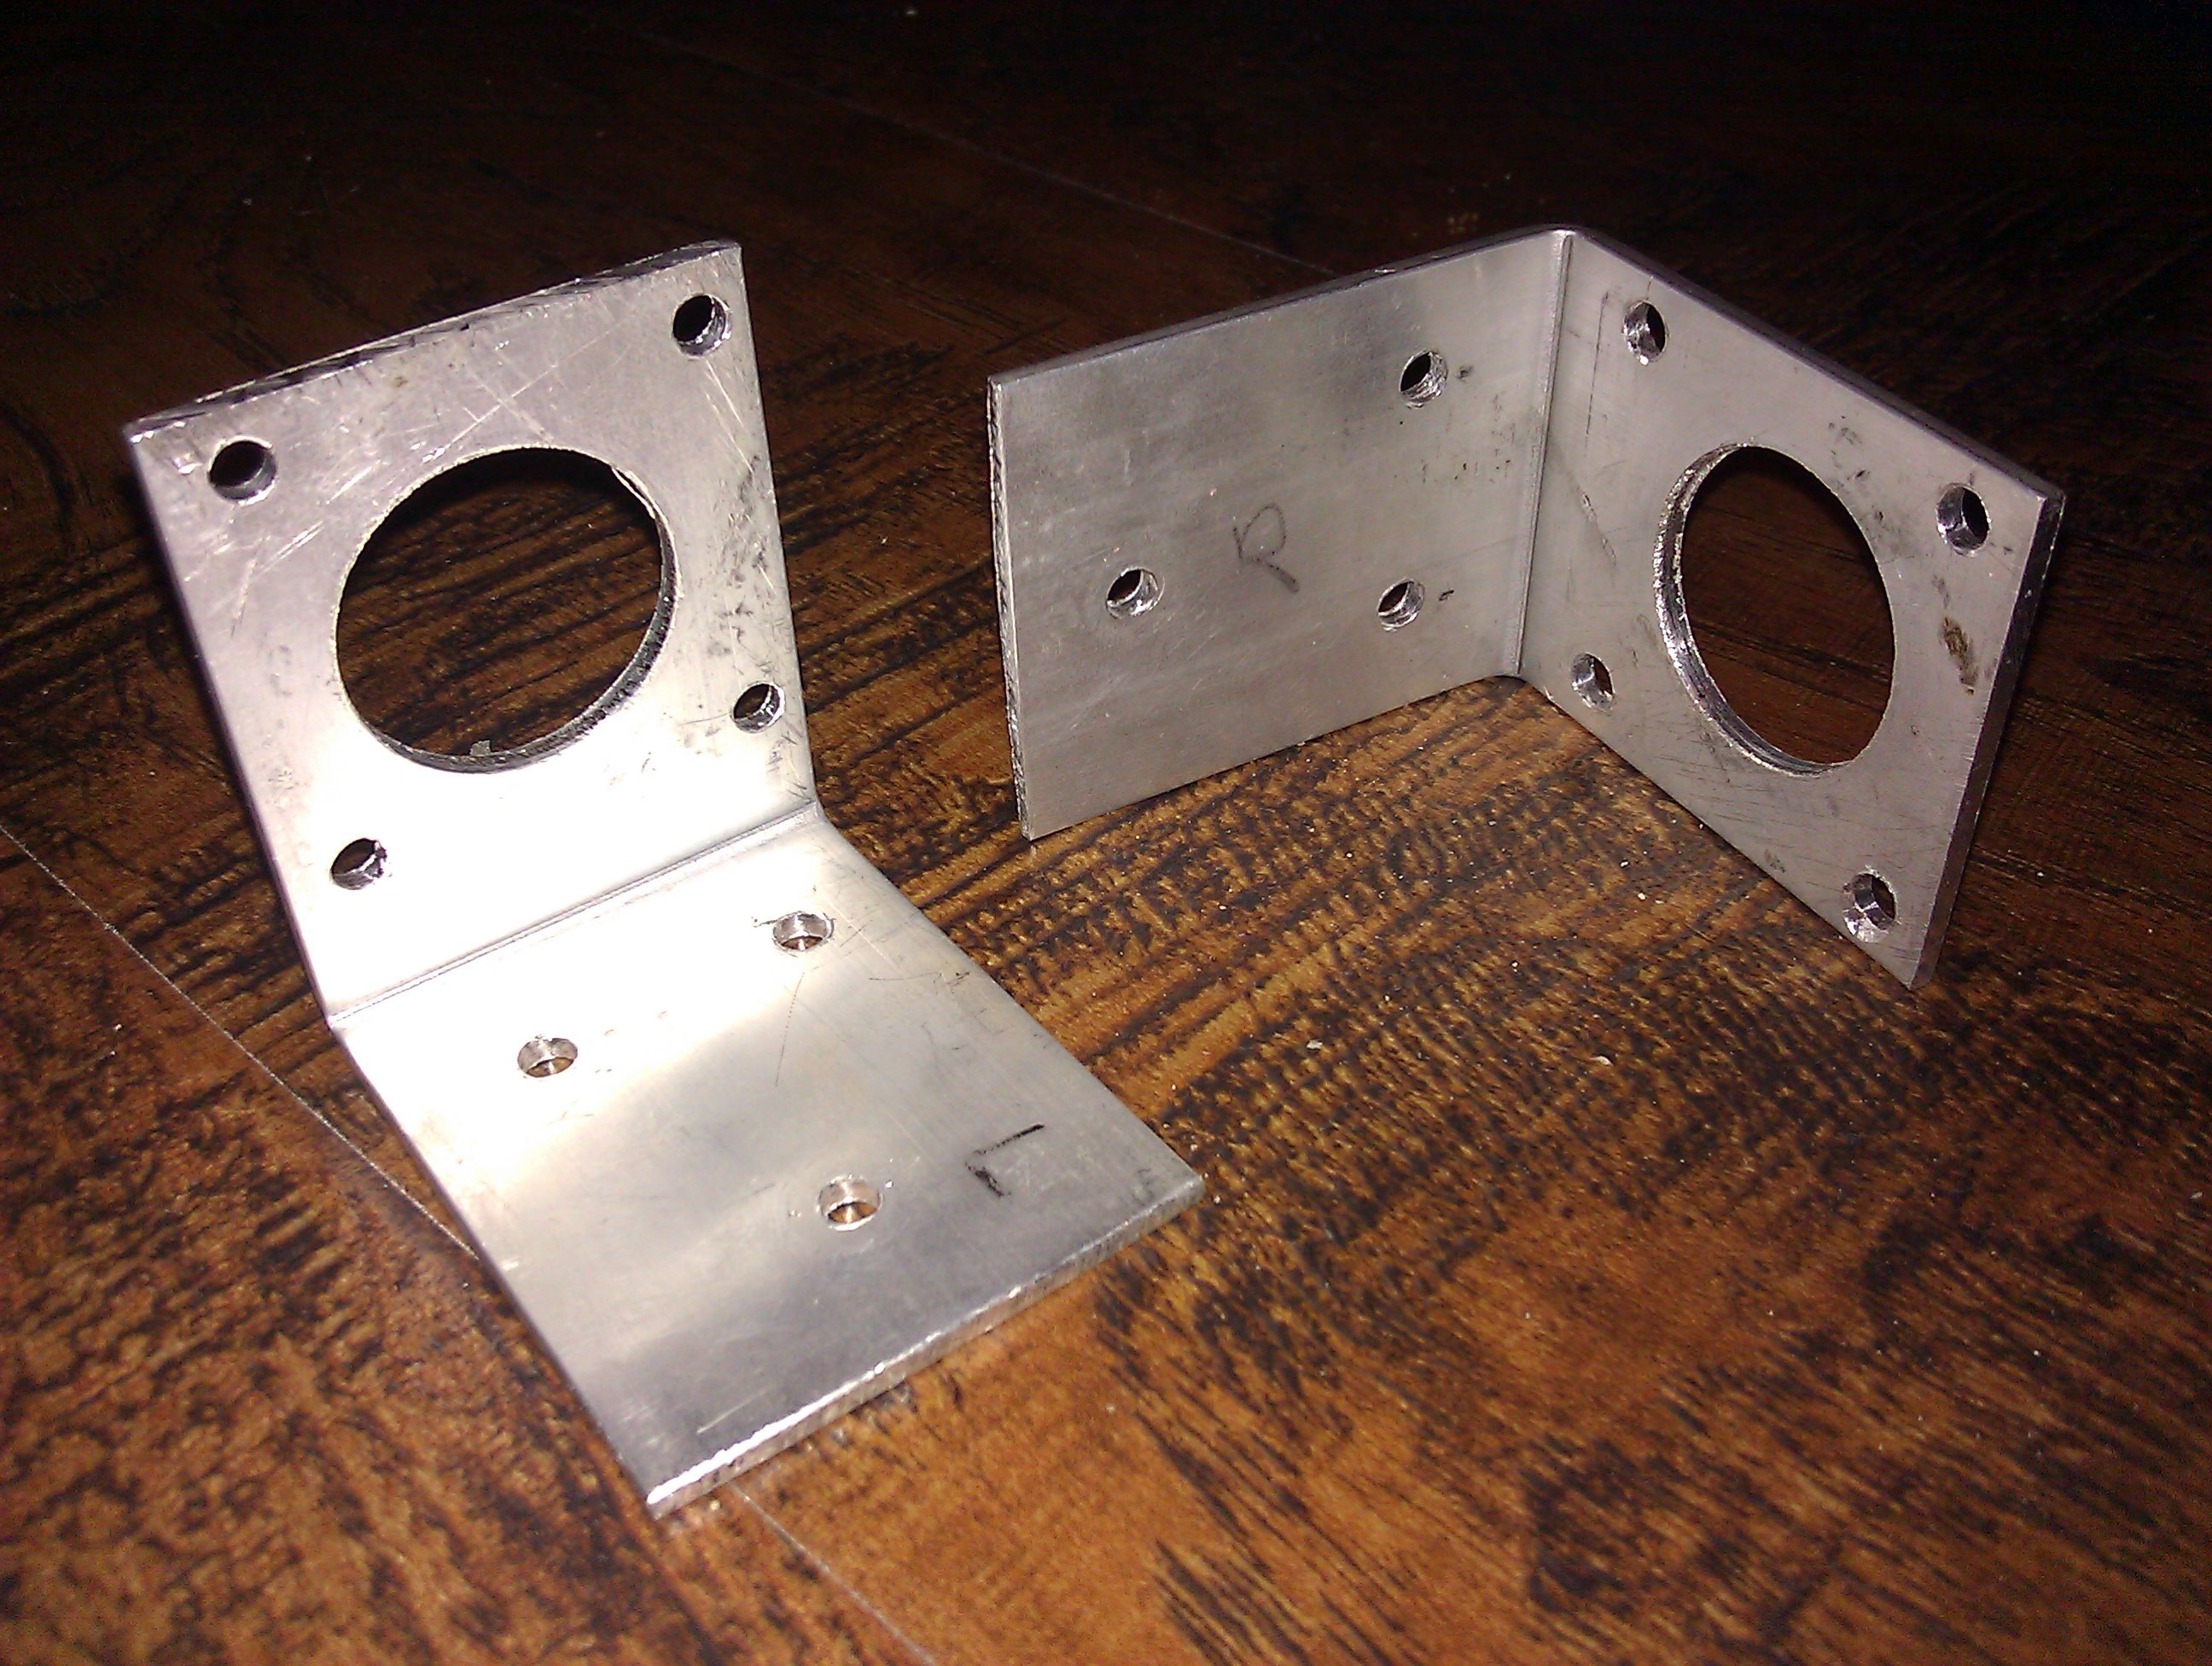
\includegraphics[width=3.0in]  {Images/motor-mount-1.jpg}
        \caption{Motor Mounts}
        \label{Motor Mounts}
\end{figure}
These mounts are just the cut strips of aluminium that have been bent so that they form a 90 degree angle and holes drilled through them to accommodate the motor drive shaft and for screw holes to attach these mounts to the baseplate.
\\Another alteration to the original design is the fact that I have chosen to use only two drive wheels instead of the four shown in the design document.  The reasoning for this was that it is easier to turn with just the two wheels as it will be able to almost turn on the spot rather than having to perform a multi directional turn, moving backwards and forwards turning a different direction for each just like how a driver would turn a car around in a tight space.  Also the kit used in the prototype only used two drive wheels with a caster wheel for stability and was in fact very stable, more than stable enough for this project and removes some complexity from the drive system.
\begin{figure}[H]
\centering
        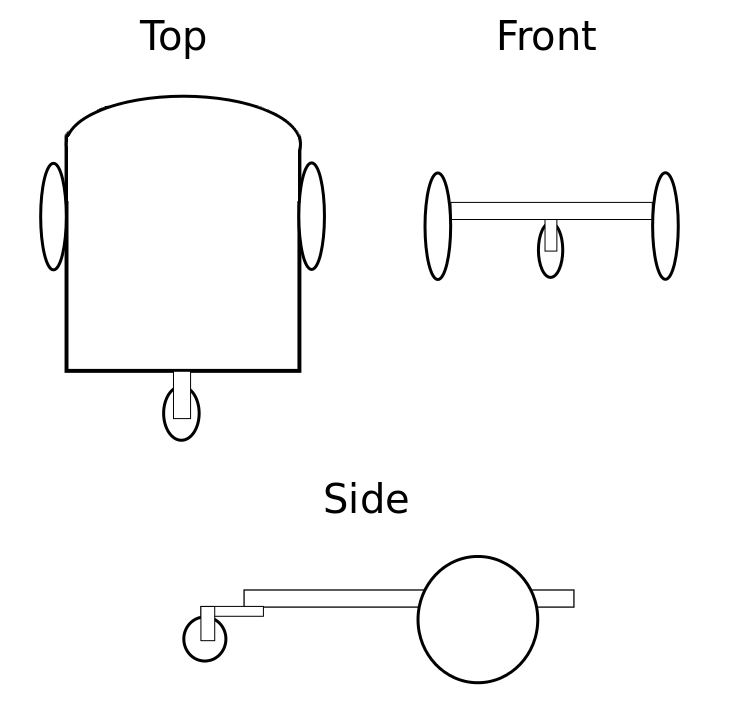
\includegraphics[width=4.0in]  {Images/second-design.png}
        \caption{Two Wheel Drive Design}
        \label{Two Wheel Drive Design}
\end{figure}
Now that the design has been reduced from four drive motors down to only two it will need some other wheels to keep the robot stable.  A single rear caster wheel worked well for the prototype and if I went with two rear stabilising wheels then the car turning in a tight space issue would still apply and because of this a single wheel has been chosen.
\\This wheel again has been mounted on a strip of aluminium bolted hanging over the rear end of the also aluminium baseplate.
\begin{figure}[H]
\centering
        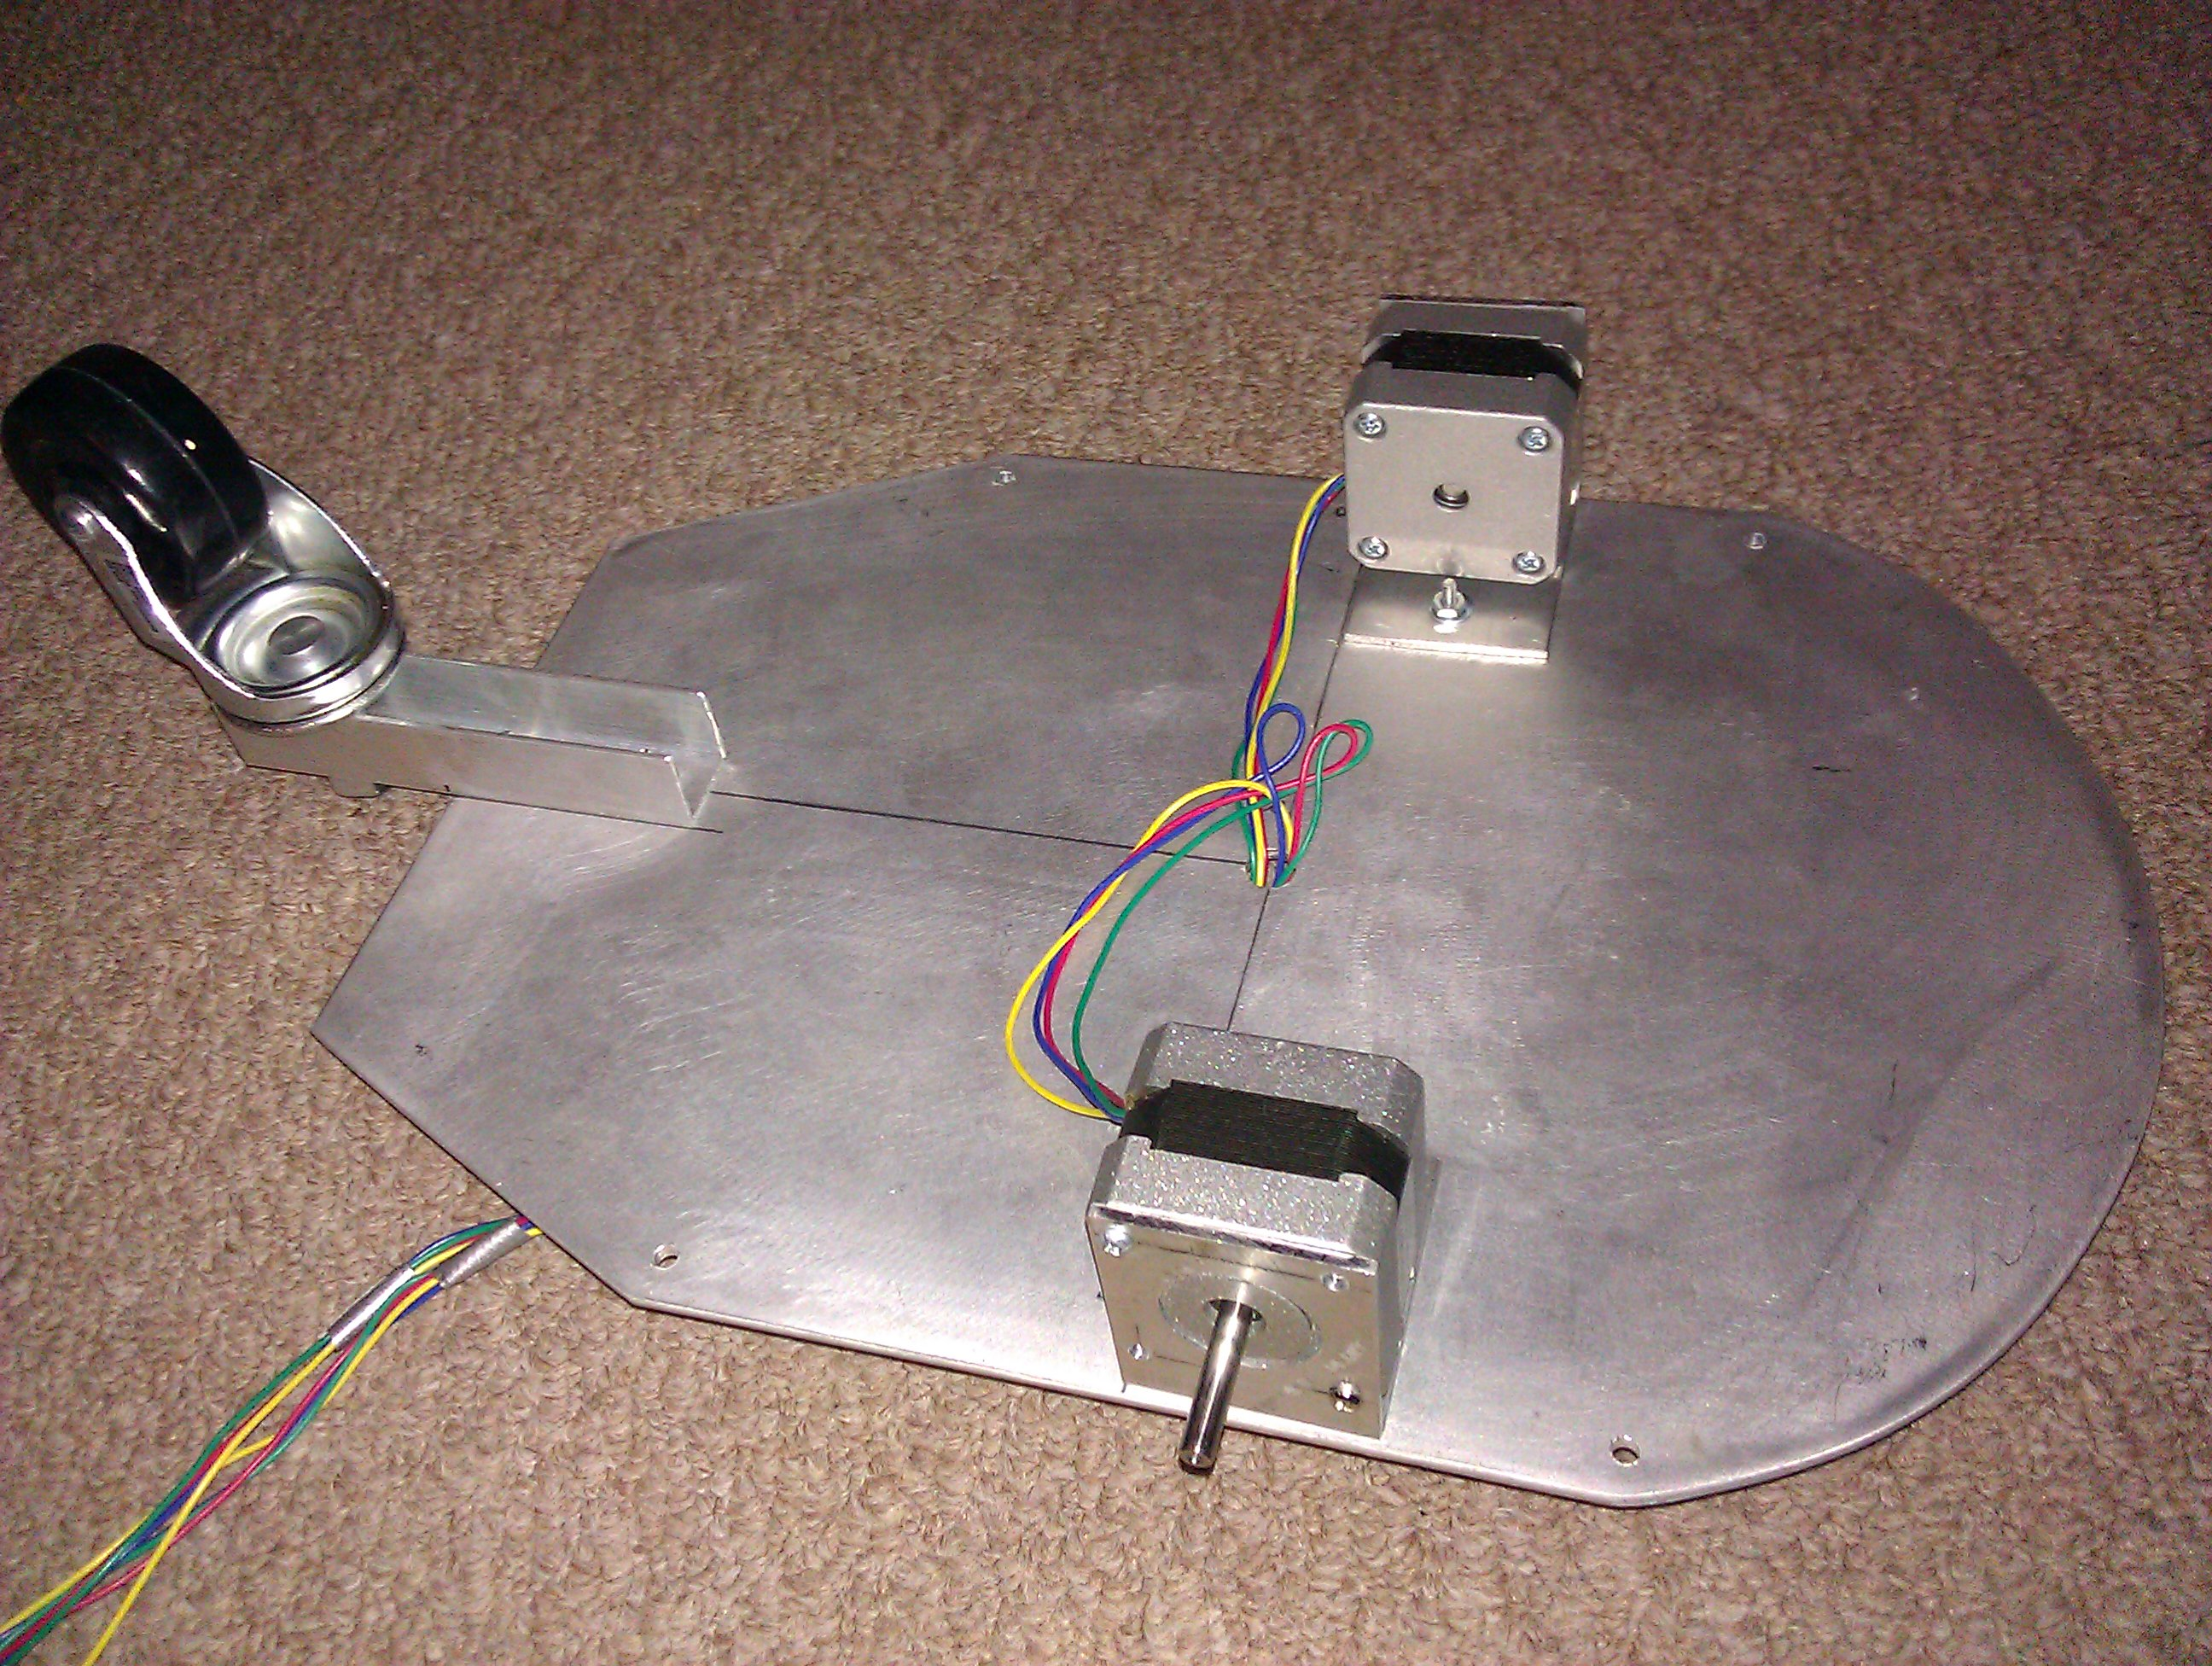
\includegraphics[width=3.0in]  {Images/baseplate-underside.jpg}
        \caption{Baseplate Underside}
        \label{Baseplate Underside}
\end{figure}
Next was to attach the stepper motors to the cut out motor mounting plates and attach the chosen off road wheels to them.  The wheels are attached to the motor shaft with the use of a hollow shaft attached to the wheel and a grub screw through that hollow shaft to clamp onto a flat edge that I cut into the motor shaft for grip.
\subsection{Manufacturing Parts}
Before starting this project I spent some time building a three dimensional printer.  This device is just like an ordinary printer but creates three dimensional physical objects.
\\An ordinary printer uses a print head to dispense ink onto a sheet or paper or card to leave a permanent mark on it which after a lot of small applications of the ink will build up letters or a picture.  A three dimensional printer works in a very similar way.  Plastic is fed into the print head where it is heated up above the melting point of whichever plastic is being used then extruded out onto a heated print bed.  While this melted plastic is being extruded the head is being moved around to draw out the shape of whatever is being printed.  This is currently still essentially two dimensional, what happens next is that once the first layer is finished with either the print head moves up or the print bed moves down and the next layer is started.  This is how this type of printer works, after the first layer is printed onto the heated bed, the next layer is printed on top of the previous one.  This process continues as many times as necessary until the layers are built up into the full object.
\\This process is very useful as it wastes no materials as it is an additive process as opposed to other computer aided manufacturing methods which are generally subtractive.  This means that other machines cut away excess off of a block of a selected material when this printer only adds material that is needed.
\\The reason I built this printer is to produce one off custom components for any project I might need such a capability.  Instead of trying to source the exact component I want of the right size and shape, or having to modify something else, the idea of just being able to create a three dimensional model on a computer of the object I want to create and then just be able to make it at a whim is a very attractive prospect.  These parts do not only have to be plastic, there are 3D printers can can even print metal, some of these parts are used in aircraft\cite{mitprint} and even formula one\cite{f1print} cars.  These parts were made using a power type 3D printer which uses the same concept as the printers available for consumer purchase but instead of extruding melted plastic from a heated nozzle they use an extremely fine powder which is dusted over the print area and melted in the correct areas with lasers.
\begin{figure}[H]
\centering
        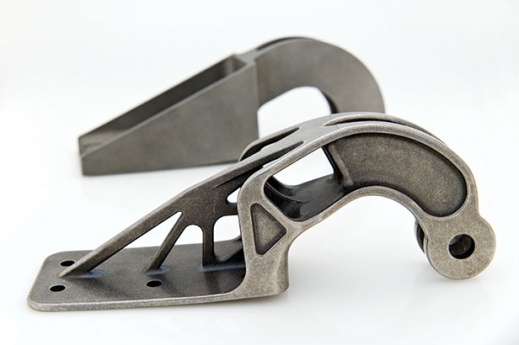
\includegraphics[width=4.0in]  {Images/print-aircraft.jpg}
        \caption{3D Printed Aircraft Part - technologyreview.com}
        \label{3D Printed Aircraft part}
\end{figure}

The printer I built had many printed components as parts of its own construction.  These parts were made out of a blue plastic. This printer was bought in kit form from a company called Felix Printers\cite{felix} in the Netherlands and took about a day to construct and a further day to configure and get working to an acceptable quality of parts produced by it.
\begin{figure}[H]
\centering
        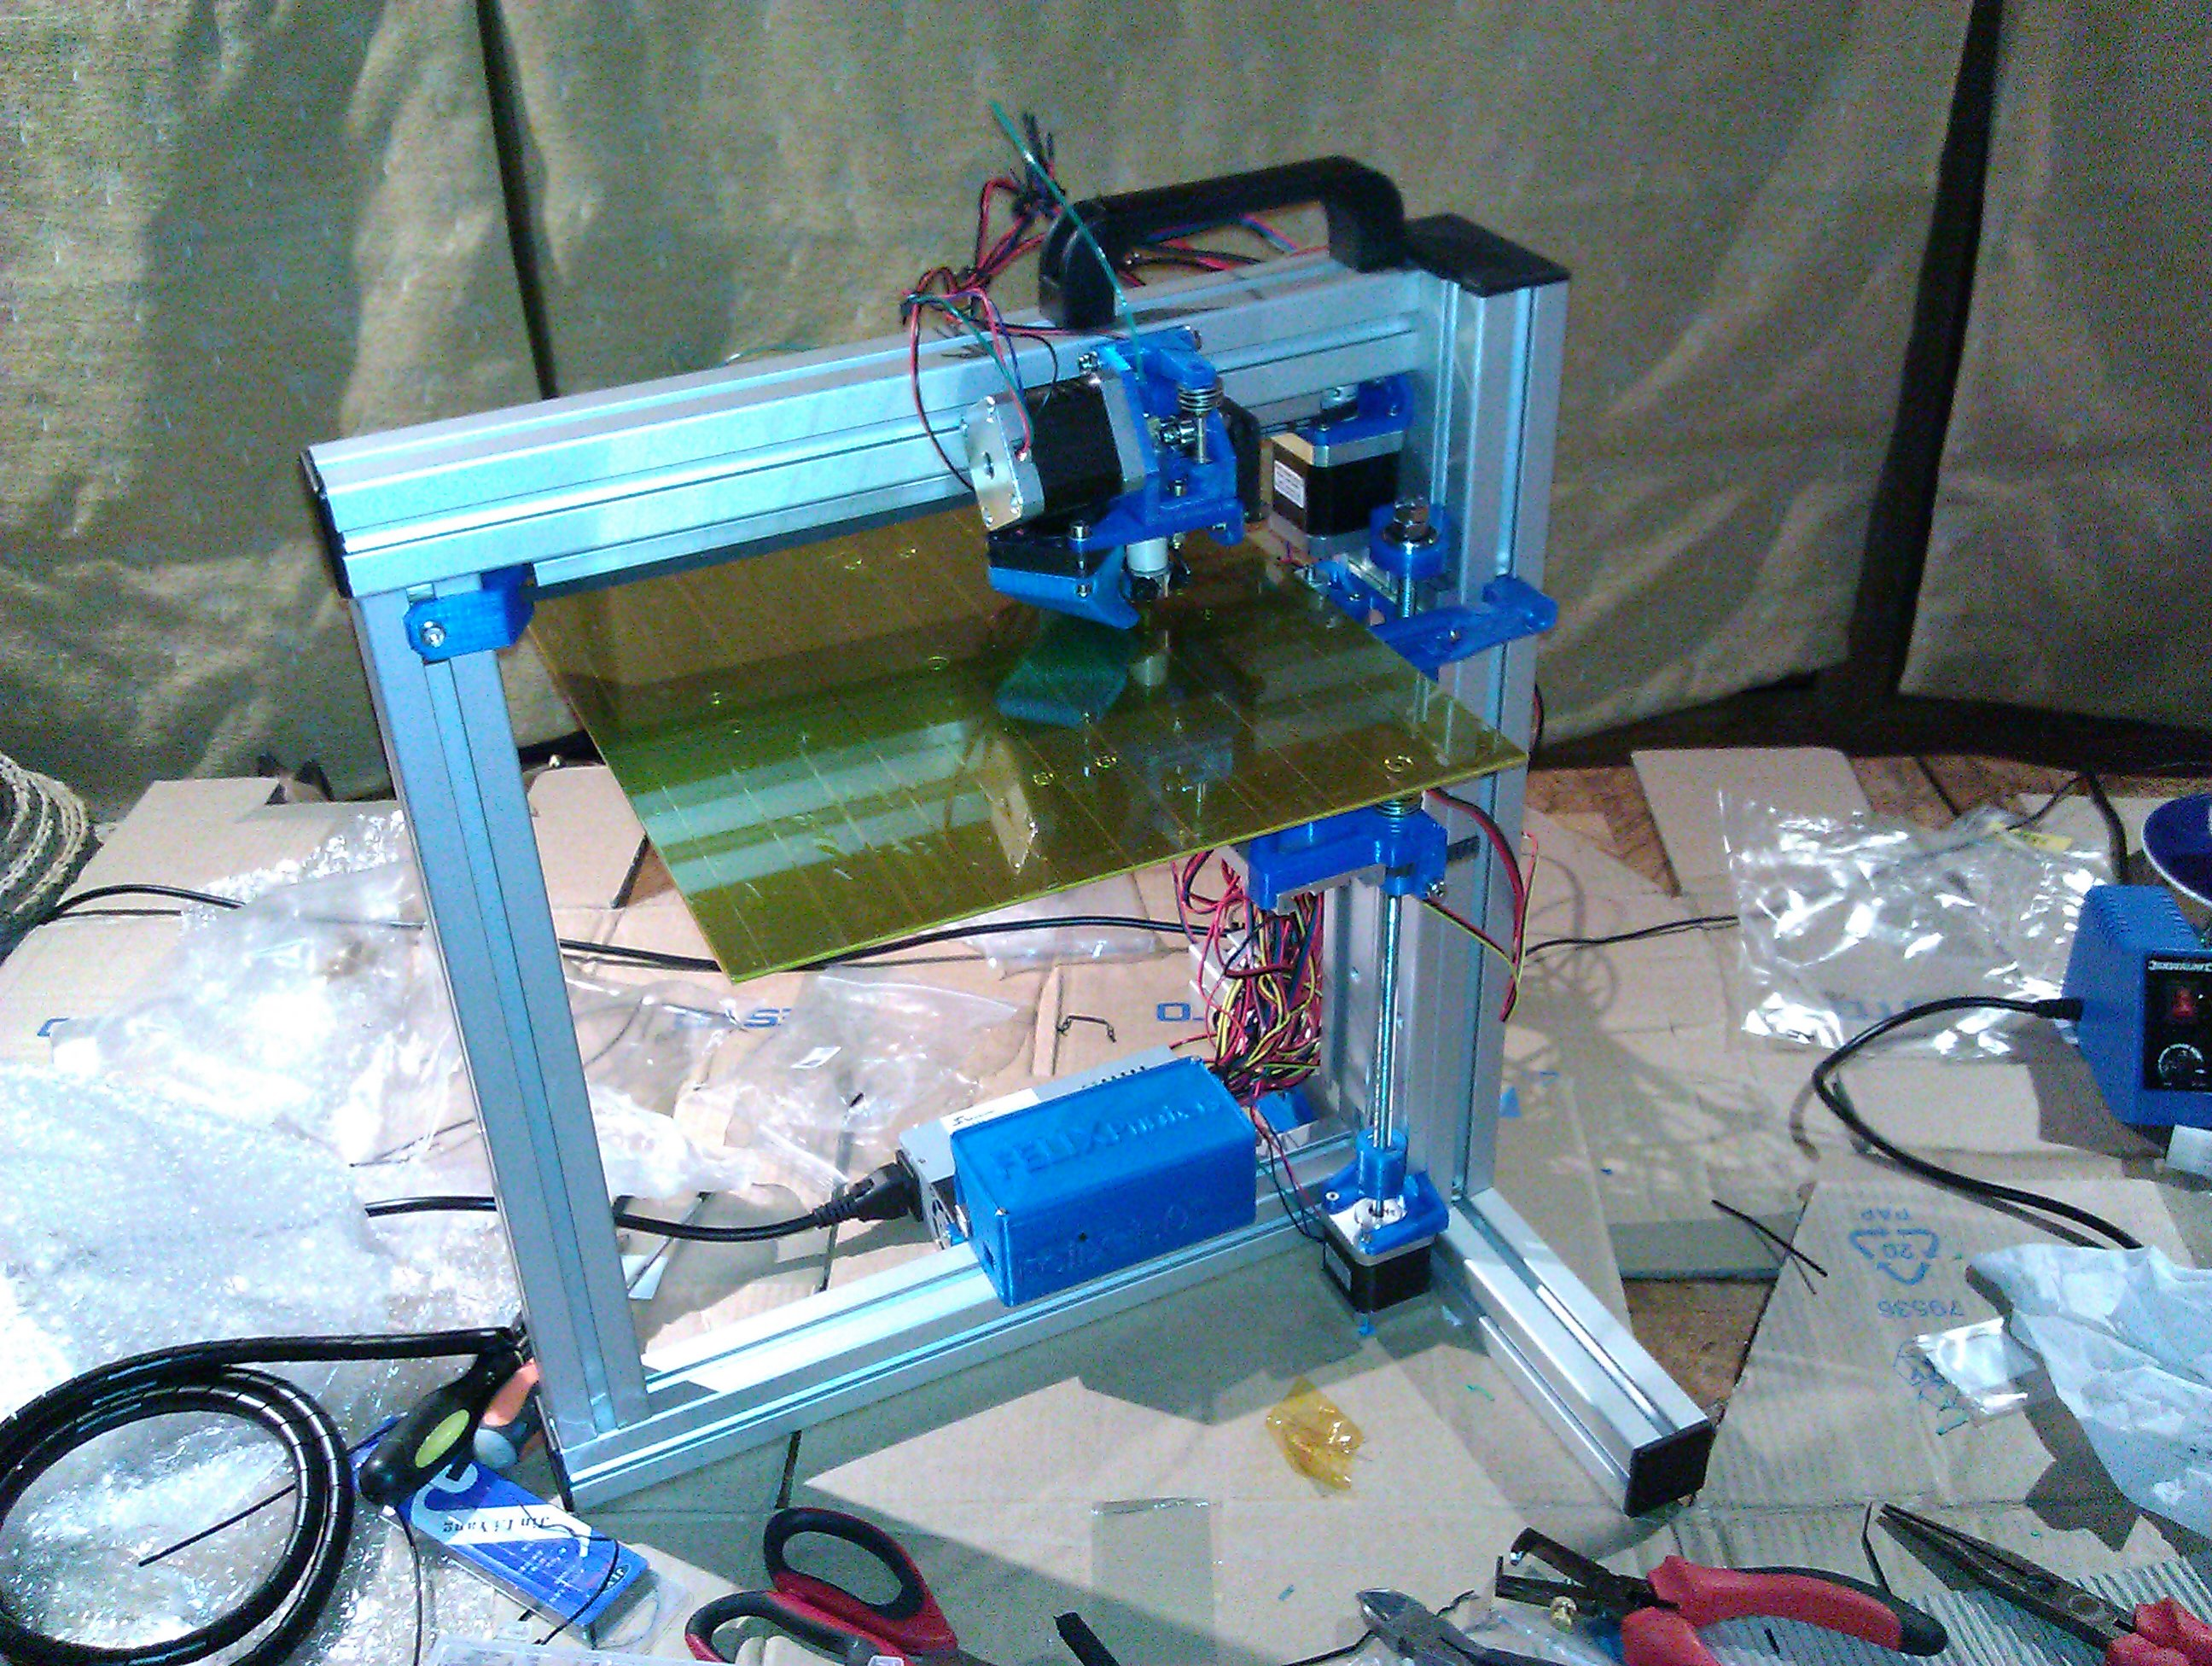
\includegraphics[width=5.0in]  {Images/printer.jpg}
        \caption{3D Printer}
        \label{3D Printer}
\end{figure}
The first component for the robot that I constructed with this printer is a mount for the microcontroller.  The mount is use to attach the component to the chassis and to insulate it from the metal base to avoid short circuits between varies part of the component and between it and other components that may also be mounted on the same base plate.  This mounting plate was constructed by the printer in less than half an hour and weighing under 25 grams and costing me less than 50 pence.
\begin{figure}[H]
\centering
        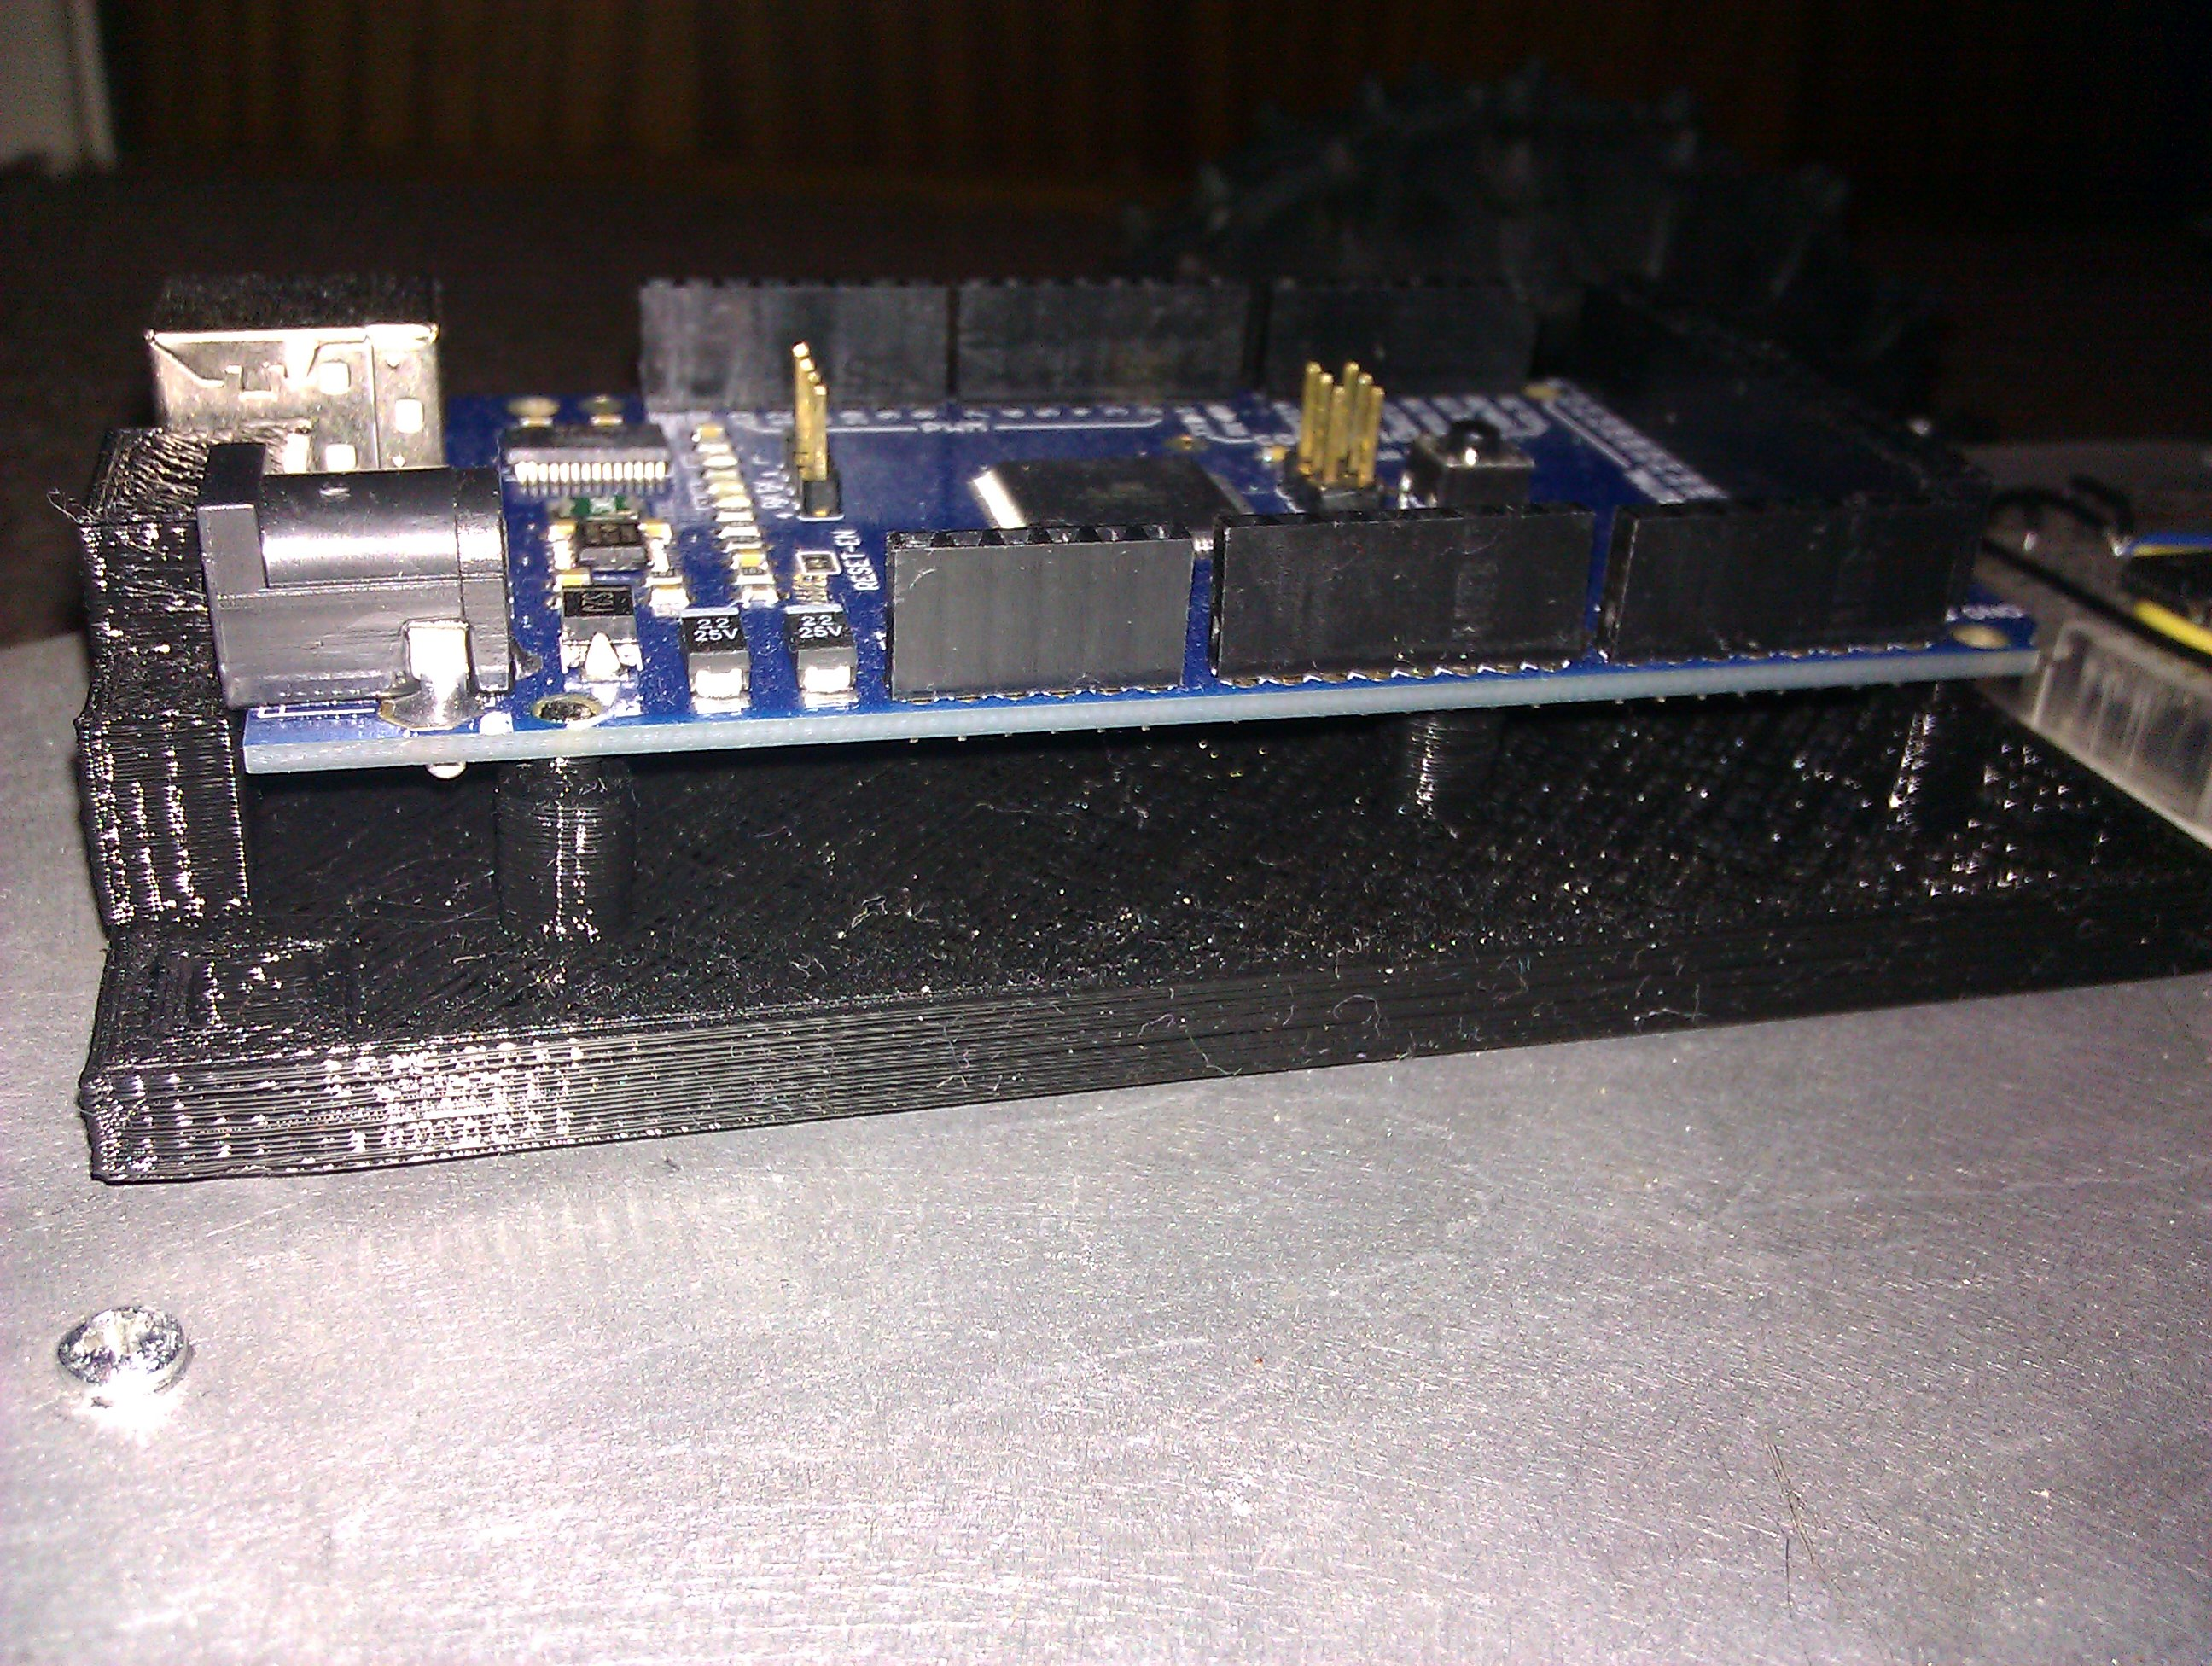
\includegraphics[width=5.0in]  {Images/printed-mount.jpg}
        \caption{Printed Mounting Plate}
        \label{Printed Mounting Plate}
\end{figure}
Eventually the printed mounting plate will be attached to the base plate with bolts but at this stage of development it is just help in place with adhesive tape.  There is a prototyping breadboard used for the h-bridge motor driver also fixed in place with the adhesive tape. With the drive wheels attached to the motors and mounted to the base plate, the rear caster wheel set in place, the Arduino microcontroller and the motor driver breadboard taped to the base plate it was ready to test the drive system.
\begin{figure}[H]
\centering
        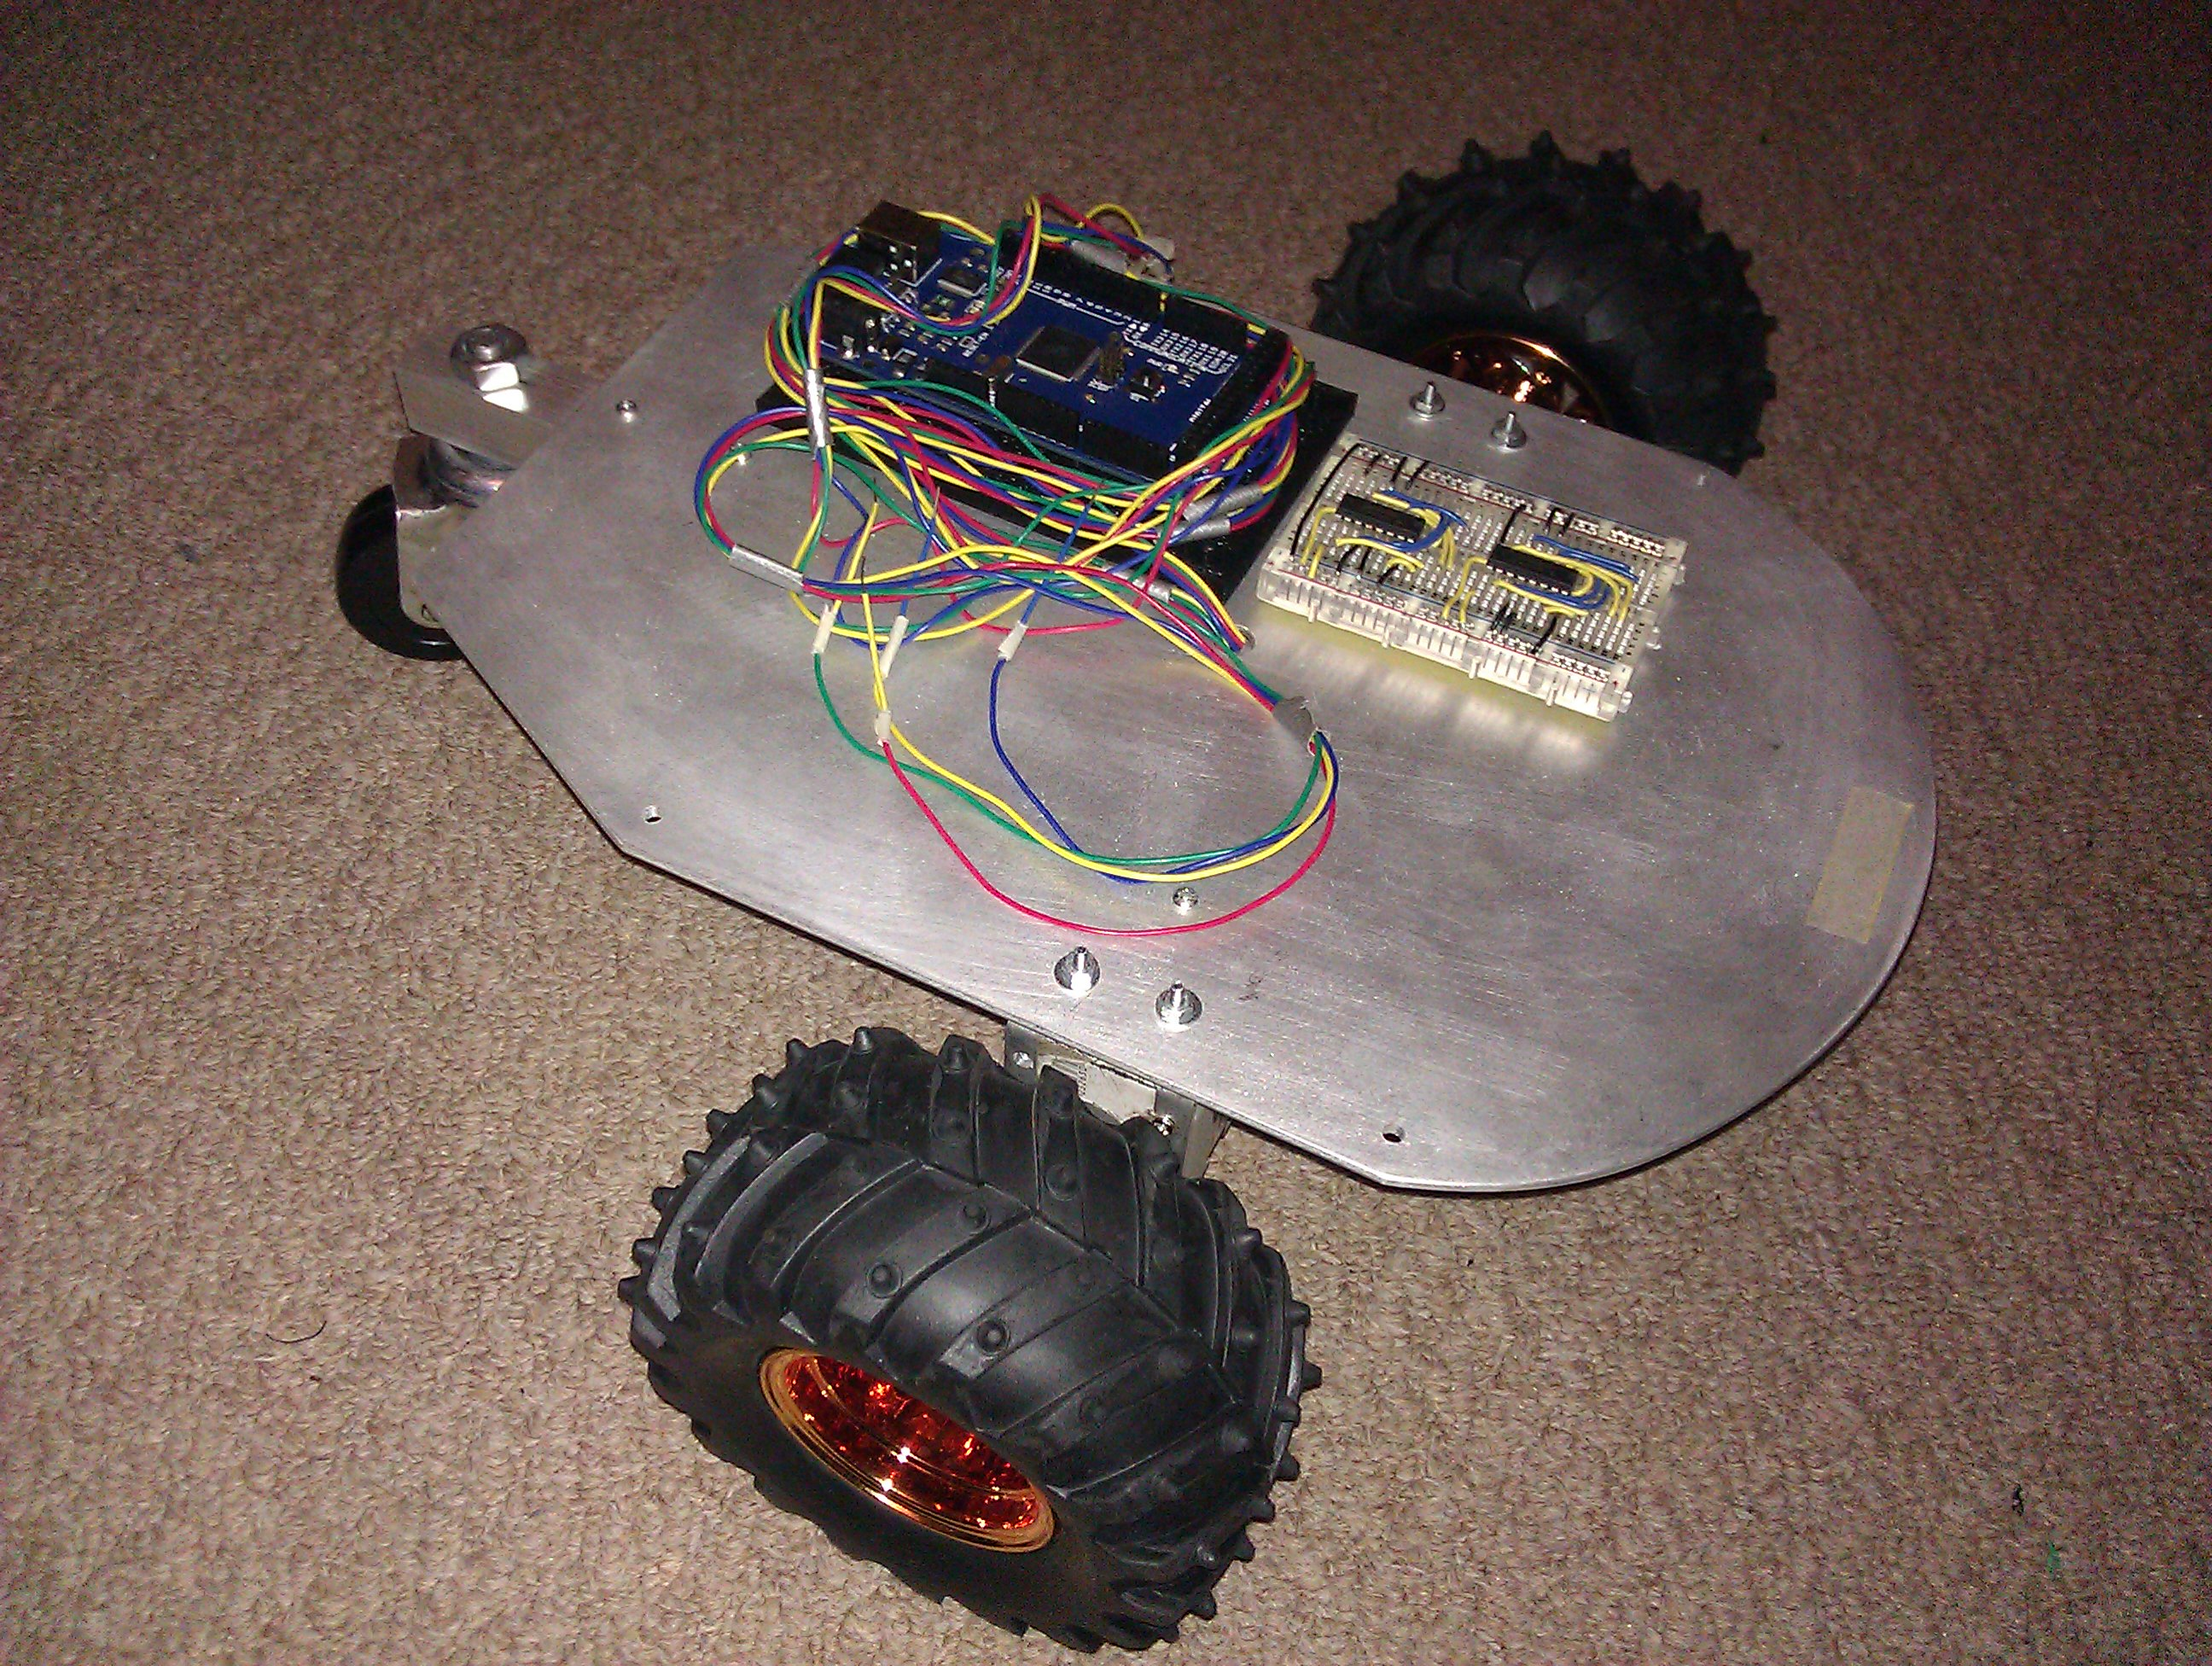
\includegraphics[width=5.0in]  {Images/tria-mkII.jpg}
        \caption{Completed MK-I}
        \label{Completed MK-I}
\end{figure}
